\documentclass{Exams}
\usepackage{preamble}
\usepackage{fancyhdr}
\pagestyle{fancy}

%   Используйте для теоремы окружение 
%   \begin{theorem}[name] \end{theorem}
%   Аналогично:
%   определение (definition)
%   лемма (lemma),
%   следствие (corollary)
%   пример (example)
%   замечание (remark)
%   док-во (Proof) (именно с большой буквы)

% \Nat - множество натуральных чисел
% \Real - множество вещественных чисе
% \Zint - множество целых чисел
% \Complex - множество комплексных чисел
% \eps - эпсилон  
\fancyhead[RO]{\slshape Д. Дружкин, А. Орехова, А. Стюхина, В. Янченко \rightmark}
\fancyfoot[C]{\thepage}

\author{}
\title{Билеты к зачету}
\date{2023}
\begin{document}

\subject{Алгем}
\ExamMakeTitle
\section*{Системы линейных уравнений}
\input{Linear_equations.tex}

\section*{Определители и их приложения}
\subsection*{Линейные формы}
\begin{definition}
  \textit{Линейной функцией} или \textit{линейной формой} на векторном пространстве $V$ называется функция $\alpha:\; V \to \Real$ (в общем виде $\alpha:\; V \to K$, где $K$ "--- поле), обладающая следующими свойствами:
  \begin{enumerate}
    \item $\alpha(\bar{x} + \bar{y}) = \alpha(\bar{x}) + \alpha(\bar{y})$
    \item $\alpha(\lambda\bar{x}) = \lambda\alpha(\bar{x})$
  \end{enumerate}
\end{definition}
\begin{definition}
  \textit{Билинейной функцией} или \textit{билинейной формой} на векторном пространстве $V$ называется форма $\alpha: V \times V \to \Real$ (паре векторов сопоставляется действительное число), линейная по каждому аргументу, то есть:
  \begin{enumerate}
    \item $\alpha(\lambda_1\bar{x}_1 + \lambda_2\bar{x}_2,\,\bar{y}) = \lambda_1\alpha(\bar{x}_1,\,\bar{y}) + \lambda_2\alpha(\bar{x}_2,\,\bar{y})$
    \item $\alpha(\bar{x}, \gamma_1\bar{y}_1 + \gamma_2\bar{y}_2) = \gamma_1\alpha(\bar{x},\bar{y}_1) + \gamma_2\alpha(\bar{x},\bar{y}_2)$
  \end{enumerate}
\end{definition}
\begin{example}
  Самый наглядный пример билинейной функции "--- скалярное произведение.

  Для любых функций $f(x)$ и $g(x)$, интегрируемых на отрезке $[a,b]$, функция $I(f,g) = \int\limits_a^b{f(x)g(x)\,\mathrm{d}x}$ является билинейной функцией на $[a,b]$.
\end{example}
\begin{definition}
  \textit{Скалярным произведением} называется билинейная форма, обладающая свойствами:
  \begin{enumerate}
    \item Симметричность $(\bar{x},\bar{y}) = (\bar{y},\bar{x})$
    \item Положительная определённость $(\bar{x},\bar{x}) > 0$ и $(\bar{x},\bar{x}) = 0 \Leftrightarrow \bar{x} = \bar{0}$
  \end{enumerate}
\end{definition}

\subsection*{Определитель матрицы $n$"=ого порядка}

Пусть $V$ "--- действительное пространство, функция $f\!: \underbrace{V \times \ldots \times V}_{m} \to \Real$.
\begin{definition}
  Функция $f$ называется \textit{полилинейной}, если она линейна по каждому аргументу.
\end{definition}
\begin{definition}
  Полилинейная функция называется \textit{кососимметрической}, если при перестановке любых двух аргументов она умножается на $-1$.
\end{definition}

\begin{definition}
  \textit{Определителем} квадратной матрицы $A = (a_j^i),~ i,\,j = 1,\ldots,n$ называется число $$det\;A = \sum\limits_{k_1, k_2, \ldots, k_n}sgn(k_1, \ldots, k_n) \cdot a_{k_1}^1 \, a_{k_2}^2 \ldots a_{k_n}^n, $$
  где $sgn(k_1, \ldots, k_n)$ "--- знак перестановки.
\end{definition}

\begin{theorem}
  Определитель является кососимметрической полилинейной функцией строк матрицы 
  
  Всякая функция $f$ на множестве квадратных матриц порядка $n$, являющаяся кососимметрической полилинейной функцией строк матрицы имеет вид
  $f(A) = f(E) \cdot det\;A$ в частности, если $f(E) = 1$, то $f(A) = det\;A$.
\end{theorem}

\begin{definition}
  Матрица $A$ называется \textit{невырожденной}, если определитель матрицы $A$ не равен нулю. ($det\; A \neq 0)$.
\end{definition}
\begin{theorem}[об определителе матрицы с углом нулей]
  Пусть $A = \begin{pmatrix}
    B & D \\
    0 & C
  \end{pmatrix}$, где $B$ и $C$ квадратные матрицы. Тогда $det\;B \cdot det\;C = det\;A$.
\end{theorem}

\begin{lemma}
  $\begin{vmatrix}
    a_1^1 & \ldots & a_j^1 & \ldots & a_n^1 \\
    0 & 0 & a_j^i & 0 & 0 \\
    \vdots& \ldots& \vdots & \ldots & \vdots \\
    a_1^n & \ldots & a_j^n & \ldots & a_n^n 
  \end{vmatrix} = A_j^i \, \cdot \, a_j^i$, где $A_j^i$ "--- алгебраическое дополнение элемента $a_j^i$ и вычисляется $A_j^i = (-1)^{i + j} \cdot M_j^i$. 
  
  $M_j^i$ "--- минор элемента $a_j^i$.
\end{lemma}
\begin{Proof}
  Переставляя строки и столбцы приведем матрицу к виду:
  $$
  \left(\begin{array}{cccc}
    \textcolor{red}{a_j^i} & 0 & \ldots & 0 \\
    a_j^1 & \textcolor{blue}{a_1^1} & \textcolor{blue}{\ldots} & \textcolor{blue}{a_n^1} \\
    \vdots & \textcolor{blue}{\vdots} & \textcolor{blue}{\ddots} & \textcolor{blue}{\vdots} \\
    a_j^n & \textcolor{blue}{a_1^n} & \textcolor{blue}{\ldots} & \textcolor{blue}{a_n^n}
  \end{array}\right) = det\;B \cdot det\;C = a_j^i \cdot det\;C = a_j^i A_j^i.
  $$ 
  (красным отмечена матрица $B$, синим "--- $C$).
\end{Proof}

\subsection*{Некоторые приложения определителя}
\begin{theorem}[Крамера]
  Если определитель матрицы коэффициентов $A$ отличен от нуля, то система 
  $$\begin{cases}
    a_1^1x_1 +  a_1^2x_2 + \ldots + a_n^1x_n = b_1 \\
    a_1^2x_1 +  a_2^2x_2 + \ldots + a_n^2x_n = b_2 \\
    ~\vdots \\
    a_1^nx_1 +  a_2^nx_2 + \dots + a_n^nx_n = b_n,
\end{cases}$$
  имеет единственное решение.

  Причем $x_i = \frac{det\;A_i}{det\;A},~ i = 1,\ldots,n$, где $A_i$ "--- матрица $A$, в которой $i$ столбец заменяется на $B = \begin{pmatrix}
    b_1\\
    \vdots\\
    b_n
  \end{pmatrix}$.
\end{theorem}
\begin{Proof}
  При элементарных преобразованиях системы уравнений в матрицах $A$ и $A_i$ происходит элементарные преобразования строк, следовательно формула Крамера не меняется.

  Рассмотрим случай, когда $A = E$. Тогда система имеет вид: $$\begin{cases}
    x_1 = b_1 \\
    ~ \vdots \\
    x_n = b_n
  \end{cases}$$

  \begin{equation*}
    det\; A_i = 
    \begin{gmatrix}[b]
    1 & 0 & \cdots & b_1 & 0 & \cdots & 0 \\
    0 & 1 & \cdots & b_2 & 0 & \cdots & 0 \\
    \vdots & \cdots & \cdots & \vdots & \cdots &\cdots & \vdots \\
    0 & 0 & \cdots & b_n & 0 &  \cdots & 1 
    \colops
    \mult{3}{\begin{array}{c}\text{i столбец}\\\downarrow\end{array}}
   \end{gmatrix} = b_i
\end{equation*}
   $\implies x_i = \frac{b_i}{1} = b_i \implies$ Формула Крамера верна.

   Если $det\; A = 0,~ \exists i:~ det\;A_i = 0 \implies$ система несовместна.

   Если $det\;A = \ldots = det\;A_n = 0 \implies$ система несовместна или неопределена.
\end{Proof}

\begin{theorem}
  Пусть $A$ "--- невырожденная квадратная матрица. Тогда \begin{equation*}
    A^{-1} = \frac{1}{det\;A} \; \begin{Vmatrix}
      A_1^1& A_1^2 & \ldots & A_1^n \\
      A_2^1 & A_2^2 & \ldots & A_2^n \\
      \vdots & \vdots & \ldots & \vdots \\
      A_n^1 & A_n^2 & \ldots & A_n^n
    \end{Vmatrix}
  \end{equation*}
  (обратите внимание, что матрица транспонирована).
\end{theorem}

\begin{Proof}
  $A \cdot A^{-1} = A^{-1} \cdot A = E$

  $\underbrace{AX = E}_{\substack{\text{Уравнение относительно} \\ \text{столбцов матрицы } X}}\implies X = A^{-1}$, то есть $A \cdot X_j = E_j$

  Эта система $n$ линейных уравнений относительно элементов $x_j^1, \, x_j^2, \ldots,\, x_j^n$.

  По формулам Крамера получим:
  \begin{equation*}
    x_j^i = \frac{1}{det\;A}\, \begin{vmatrix}
      a_1^1 & \cdots & 0 & \cdots & a_n^1 \\
      a_2^1 & \cdots & 0 & \cdots & a_n^2 \\
      \vdots && \vdots && \vdots \\
      a_1^j & \cdots & 1 & \cdots & a_n^j \\
      \vdots && \vdots && \vdots \\
      a_n^1 & \cdots & 0 & \cdots & a_n^n
    \end{vmatrix} = \frac{A_i^j}{det\;A}.
  \end{equation*}
\end{Proof}

Второй способ вычисления обратной матрицы:
$(A|E)$ приводим через элементарные преобразования к $(E|A^{-1})$
\begin{example}
  \begin{gather*}
    \begin{pmatrix}
       a_1^1 & a_2^1 \\ 
       a_1^2 & a_2^2
    \end{pmatrix} \cdot
    \begin{pmatrix} 
      x_1^1 & x_2^1 \\ 
      x_1^2 & x_2^2
    \end{pmatrix} =
    \begin{pmatrix} 
      1 & 0 \\
      0 & 1
    \end{pmatrix} \\
    \begin{pmatrix}
      a_1^1 & a_2^1 \\ 
      a_1^2 & a_2^2
   \end{pmatrix} \cdot
   \begin{pmatrix}
    x_1^1 \\
    x_1^2
   \end{pmatrix} = 
   \begin{pmatrix}
    1 \\ 0
   \end{pmatrix} \\
   \text{Например, }
   \begin{pmatrix}
    1 & 2\\
    3 & 4
   \end{pmatrix} \cdot
   \begin{pmatrix}
    x_1^1 \\ x_1^2
   \end{pmatrix} = 
   \begin{pmatrix}
    1 \\ 0
   \end{pmatrix} \\ 
   \left(\begin{array}{cc|c}
    1 & 2 & 1 \\
    3 & 4 & 0
   \end{array}\right) \thicksim 
   \left(\begin{array}{cc|c}
    1 & 2 & 1 \\
    0 & -2 & -3
   \end{array}\right) \thicksim 
   \left(\begin{array}{cc|c}
    1 & 0 & -2 \\
    0 & -2 & -3
   \end{array}\right) \thicksim 
   \left(\begin{array}{cc|c}
    1 & 0 & -2 \\
    0 & 1 & 3/2
   \end{array}\right) \\
   \begin{cases}
    x_1^1 = -2 \\
    x_1^2 = 3 / 2
   \end{cases} \\
   \text{Аналогично с вторым столбцом матрицы } X.
  \end{gather*}
\end{example}
\subsection*{Ранг матрицы}

\begin{definition}
  \textit{Минором} $k$"=го порядка матрицы $A$ называется определитель порядка $k$, построенный из $k^2$ элементов этой матрицы, расположенныъ на пересечении произвольно выбранных $k$ строк и $k$ столбцов.
\end{definition}
\begin{definition}
  \textit{Рангом} ненулевой  матрицы $A_{n\times m}$ называется натуральное число $k:~ 1 \leq k \leq min(m,\, n)$, удовлетворяющая двум условиям:
  \begin{enumerate}
    \item У матрицы $A$ существует по крайней мере один минор $k$"=го порядка, отличный от нуля. $M_k \neq 0$.
    \item Если у матрицы $A$ существует миноры $k+1$"=го порядка, то все они равны нулю. $M_{k+1} = 0$
  \end{enumerate}
\end{definition}

\begin{definition}
  Если $rk\,A = k$, то любой её $M_k \neq 0$ называется \textit{базисным} или \textit{ранговыми}. Строки и столбцы базисного минора называются \textit{базисами}.
\end{definition}
\begin{theorem}[о базисном миноре]
  У любой матрицы $A$ всякий столбец (строка) является линейной комбинацией базисных столбцов (строк).
\end{theorem}
\begin{Proof}
  Пусть $rk\,A = k$ и $M_k$ "--- базисный минор, расположенный в левом верхнем углу.

  Построим определитель окаймляющий $M_k$, который получается добавлением $i$ строки и $j$ столбца.
  \begin{equation*}
    \Delta = \begin{vmatrix}
      a_n^1 & \cdots & a_k^1 &  a_j^1 \\
      \vdots && \vdots & \vdots \\
      a_j^k & \cdots & a_k^k  & a_j^k \\
      a_1^i & \cdots & a_k^i & a_j^i \\
    \end{vmatrix} = 0
  \end{equation*}
  (так как $rk\,A = k,~ M_k \neq 0, ~M_{k + 1} = 0$)

  Раскладывая $\Delta$ по элементам последней строки получим:
  \begin{gather*}
    a_1^i A_1^{k+1} + \ldots + a_k^i A_k^{k + 1} + a_j^i M_k = 0 \\
    a_j^i = a_1^i \frac{-A_1^{k + 1}}{M_k} + \ldots + a_k^i \frac{-A_k^{k + 1}}{M_k} \\
    a_j^i = \lambda_1 a_1^i + \ldots + \lambda_k a_k^i \\
    a_j^i \text{ линейно выражается через остальные}
  \end{gather*}
\end{Proof}



\section*{Алгебра многочленов}
(если выполнено домашнее задание, то раздел не нужно учить)
404

\section*{Группы}
\subsection*{Циклические группы}
\begin{definition}
  \textit{Группой} называется множество $G$ с операцией умножения, обладающей следующими свойствами:
  \begin{enumerate}
    \item $(ab)c = a(bc),~\forall\;a,b,c \in G$ (ассоциативность)
    \item $\exists e \in G \text{ (единица)}\!:~ ae=ea=e~\forall a \in G$
    \item $\forall a \in G~\exists a^{-1} \in G \text{ (обратный элемент)},~aa^{-1} = a^{-1}a = e$
  \end{enumerate}
\end{definition}
Группа называется \textit{абелевой} или \textit{коммутативной}, если $ab=ba,~\forall a,\;b \in G$.

В любой группе может быть определена степень элемента $g \in G$ с целыми показателями:
$$ g^k = 
\begin{cases}
  \underbrace{g \cdot g \ldots \ \cdot g}_k,& \text{если } k > 0 \\
  e,& \text{если } k = 0 \\
  \underbrace{g^{-1} \cdot g^{-1} \ldots \ \cdot g^{-1}}_k,& \text{если } k < 0 \\
\end{cases}, ~~~k \in \Zint
$$
\begin{definition}
  Степени элемента $g$ образуют подгруппу группы $G$. Она называется \textit{циклической} и обозначается $<\!g\!>$
\end{definition}
\begin{definition}
  Наименьшее из натуральных $m$ для которого выполняется $g^m = e$ называется \textit{порядком} элемента.

  Если $m$ не существует, то порядок $g$ равен $+\infty$.

  Обозначение: $ord\;g = m$.
\end{definition}
\begin{theorem}
  Если $ord\;g = n$, то 
  \begin{enumerate}
    \item $g^m = e \Leftrightarrow n \mid m$
    \item $g^k = g^l \Leftrightarrow k \equiv l (mod\; n)$ 
  \end{enumerate}
\end{theorem}
\begin{Proof}
  \begin{enumerate}
  
    \item $m = np + r,~ r < n$

  $g^m = g^{np} \cdot g^r = (\underbrace{g^n}_{e})^p \cdot g^r = g^r$

  $\Rightarrow ~ g^m = e \implies g^r = e \implies r = 0 \implies n \mid m$

  $\Leftarrow$ так как $n \mid m$, то $r = 0  \implies g^r = g^0 = e$.
  \item $g^k = g^l \implies g^{k - l} = e$
  
  $\implies$ по первому утверждению $(k - l)\;\vdots \;n \implies k \equiv l$  (mod $m$)
\end{enumerate}
\end{Proof}

В аддитивной группе говорят не о степенях элемента $g$, а о его кратных. Обозначение: $m\;g$

Порядком элемента $g$ в \textit{аддитивной} группе называют наименьшее из натуральных $m$, такое, что $\underbrace{g+g+\ldots+g}_m = 0$(если $m$ существует).
\begin{theorem}
  Если $ord\;g = n$, то $ord\;g^k = \frac{n}{(n,k)},~(n,k) = \gcd(n,k)$ (НОД($n,k$))
\end{theorem}
\begin{Proof}
  Пусть $ord\;g^k = m$ и $(n,k) = d$. Тогда $n = n_1d,~ k = k_1d, ~(n_1,k_1) =1$.

  Так как $ord\;g = n$, то $g^n = e$. Также $(g^k)^m = e \implies km\;\vdots\;n \implies k_1dm\;\vdots \; n_1d \implies k_1m \;\vdots\; n_1$
  
  Так как $(k_1,n_1) = 1 \implies m\;\vdots\;n_1 \implies m = pn_1 = \frac{pn_1d}{d} = \frac{pn}{d}$ Так как $m = ord\; g^k$, то есть наименьшее натуральное число, удовлетворяющее определению порядка, $\implies p = 1$.

  $\implies ord\;g^k = m = \frac{n}{d} = \frac{n}{(n,k)}$.
\end{Proof}

\begin{definition}
  Группа $G$ называется \textit{циклической}, если существует такой элемент степени которого образует группу $G$. 
  
  $G = <\!g\!>$ и такой элемент называется \textit{образующим}.
\end{definition}

\begin{example}
  $\Zint$ аддитивная группа целых чисел является циклической с образующим элементом $1$ или $-1$

  $Z_n$ "--- циклическая группа с образующим элементом $[1]$.
\end{example}

\begin{definition}
  Число элементов конечной группы называется её \textit{порядком}.

  Обозначение: $\mathopen|G\mathclose|$
\end{definition}
\begin{example}
  Всякая бесконечная циклическая группа изоморфна группе целых чисел:

  $f: \Zint \to G$,

  $f: k \to g^k$.

  Всякая конечная цилкическая группа порядка $n$ изоморфна группе $Z_n$:

  $f: Z_n \to G$.

  
\end{example}
\begin{theorem}
  Всякая подгруппа циклической группы является циклической. 
  
\end{theorem}

\begin{theorem}
  В циклической группе порядка $n$ порядок любой подгруппы делит $n$ и для любого делителя $p$ числа $n$ существует одна подгруппа порядка $p$.
\end{theorem}

\subsection*{Разбиение на смежные классы}

\begin{definition}
  Пусть $G$ "--- группа, $H$ "--- подгруппа группы $G$. Элементы $g_1,\; g_2 \in G$ сравнимы по модулю $H$ $(g_1 \equiv g_2~(mod\;H))$, если $g_1^{-1}g_2 \in H$.

  $g_1^{-1}g_2 = h\in H \implies g_2 = g_1h$
\end{definition}

Отношение сравнимости по модулю $H$ является отношением эквивалентности:
\begin{enumerate}
  \item \begin{gather*}
    g_1 \equiv g_1~(mod\;H)\\
    (g_1^{-1}g_1) = e \in H
  \end{gather*}
  \item \begin{gather*}
    g_1 \equiv g_2~(mod\;H) \implies g_2 \equiv g_1~(mod\;H)\\
    g_1^{-1}g_2 \in H \implies (g_1^{-1}g_2)^{-1} \in H, \text{так как является обратным}.\\
    \implies (g_2^{-1}g_1 \in H) \implies g_2 \equiv g_1~(mod\;H).
  \end{gather*}
  \item \begin{gather*}
    g_1 \equiv g_2~(mod\;H) \wedge g_2 \equiv g_3~(mod\;H)\\
    \implies g_1 \equiv g_3~(mod\;H)\\
    g_1^{-1}g_2 \in H,~ g_2^{-1}g_3 \in H\\
    \implies (g_1^{-1}\underbrace{g_2)\cdot (g_2^{-1}}_{e} g_3) \in H \implies g_1^{-1}g_3 \in H\\
    \implies g_1\equiv g_3~(mod\;H).
  \end{gather*}
\end{enumerate}

\begin{figure}[H]
  \centering
  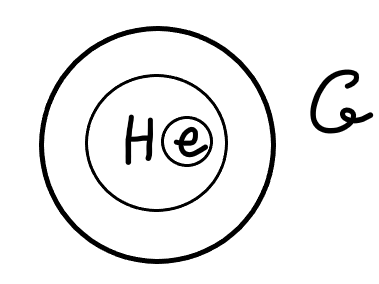
\includegraphics[height = 3cm]{images/groups_module.png}
  \caption{Пример}
\end{figure}

\begin{definition}
  Классы этой эквивалентности называются \textit{левыми смежными классами} группы $G$ подгруппы $H$.

  Смежный класс, содержащий элемент $g$, имеет вид $gH = \{gh,~h \in H\}$
\end{definition}

Одним из смежных классов является сама подгруппа $H$.

Если вместо $g_1^{-1}g_2\in H$ взять $g_2\,g_1^{-1}\in H$, то получим другое отношение эквивалентности. Классы этой эквивалентности называются \textit{правыми смежными классами}.
\begin{example}
  Смежные классы аддитивной группы $\Complex$ на подгруппе $\Real$ изображаются на комплексной плоскости прямой параллельной оси $Ox$

  $g + \Real,~g\in \Complex$

  $g + \Real = \{g + \lambda,~\lambda \in \Real\}$
  \begin{figure}[H]
    \centering
    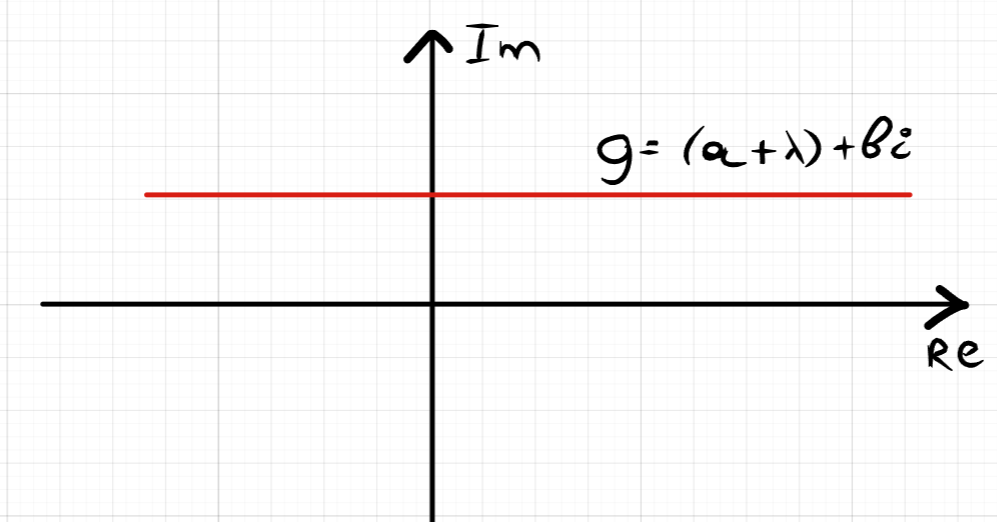
\includegraphics[height = 3cm]{images/groups_complex_example.png}
  \end{figure}
\end{example}
\begin{example}
  Смежные классы мультипликативной групп $\Complex^\ast = \Complex \setminus \{0\}$ по подгруппе $\Real^\ast_+$ изображаются на комплексной плоскости лучами, исходящими из начала координат.

  $g\Real^\ast_+ = \{g\lambda,~\lambda \in \Real\}$
  \begin{figure}[H]
    \centering
    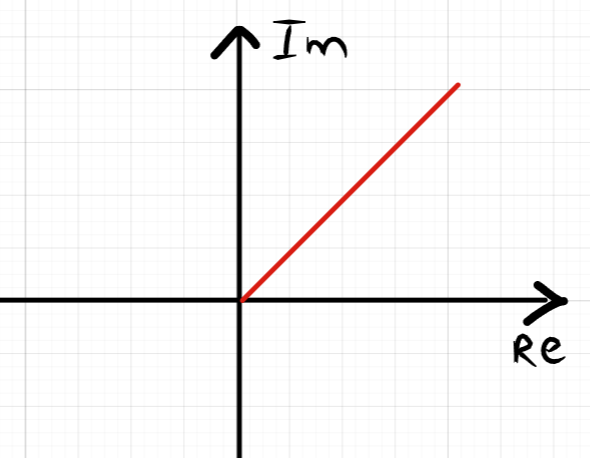
\includegraphics[height = 3cm]{images/groups_complex_withoutZero.png}
  \end{figure}
\end{example}

Множество левых смежных классов группы $G$ подгруппы $H$ обозначается $G/H$.
\begin{definition}
  Число смежных классов, если оно конечно, называется \textit{индексом} подгруппы $H$ и обозначается $\mathopen|G:H\mathclose|$.
\end{definition}
\begin{theorem}[Лагранжа]
  Если $G$ конечная группа, $H$ любая её подгруппа, то $\mathopen|G\mathclose| = \mathopen|G:H\mathclose| \cdot \mathopen|H\mathclose|$.
\end{theorem}

\begin{Proof}
  Все смежные классы $gH$ содержат одно и то же количество элементов равное $\mathopen|H\mathclose|$. Так как эти классы образуют разбиение группы $G$, то порядок группы $G$ равен произведению их числа на количество элементов подгруппы $H$ $\implies \mathopen|G\mathclose| = \mathopen|G:H\mathclose| \cdot \mathopen|H\mathclose|$.
\end{Proof}

\begin{definition}
  Подгруппа $H$ группы $G$ называется \textit{нормальной}, если $gH=Hg$, то есть $\forall g \in G:~ gHg^{-1} = H$ или $\forall g \in G, ~ \forall h \in H: ~ g \cdot h \cdot g^{-1} \in H$.

  Обозначение: $H \lhd G$, $G \rhd H$.
\end{definition}
В случае, если $H$ "--- нормальная  подгруппа группы $G$, то $G / H$ называется \textit{факторгруппой}.
$eH$ "--- единица этой группы.

\begin{definition}
  $f:~ G_1 \to G_2$ называется \textit{гомоморфизмом}, если $f(ab) = f(a)f(b),~ a,\,b \in G_1$.
\end{definition}
Свойства:
\begin{enumerate}
  \item $f(e) = e$
  \item $f(g^{-1}) = f(g)^{-1}$
  \begin{Proof}
    $f(a^{-1})f(a) = f(a^{-1}a) = f(e) = e \implies f(a^{-1}) = f(a)^{-1}$.
  \end{Proof}
  \item $Im\;f = \{f(a),~ a \in G_1\}$ "--- образ гомоморфизма. $Im\;f\subset G_2$.
  \item $Ker\;f = \{a \in G_1,~ f(a) = e\}$ "--- ядро.
  
  $Ker\;f$ есть нормальная подгруппа группа $G_1$.
  \begin{Proof}
    $a,\, b \in Ker\;f$

    $f(ab) = f(a) \cdot f(b) = e \cdot e = e \implies ab \in Ker\; f$

    $a \in Ker\; \implies f(a^{-1}) = e^{-1} = e \implies a^{-1} \in Ker\;f \implies Ker f\; \subset G_1$.

    $\forall g \in G_1,~a \in Ker\; f,~ g\,a\,g^{-1} \stackrel{?}{\in} Ker\;f$.

    $f(g\,a\,g^{-1}) = f(g)\cdot f(a)\cdot f(g^{-1}) = f(g)\cdot e \cdot f(g^{-1}) = f(g)f(g^{-1}) = f(g)(f(g))^{-1}= e$
    
    $\implies g\,a\,g^{-1} \in Ker\;f \implies Ker\; f$ есть нормальная подгруппа $G_1$.
  \end{Proof}
  \item $f(g_1) = f(g_2) \implies g_1 \equiv g_2 (mod\; Ker\;f)$
  \begin{Proof}
    $f(g_1) = f(g_2) ~/ \cdot f(g_1^{-1})$

    $f(g_1^{-1}) f(g_1) = f(g_1^{-1})f(g_2)$

    $e = f(g_1^{-1}g_2) \implies g_1^{-1}\,g_2 \in Ker\;f \implies g_1 \equiv g_2 (mod\; Ker\;f)$
  \end{Proof}
  \item $f(a^n) = (f(a))^n$
  \item $f:~ G_1 \to G_2$
  
  $\forall g \in G_1$ порядок элемента $f(g)$ делит порядок $g$.
  \begin{Proof}
    Пусть $ord\; g = k \implies g^k = e$

    $f(g^k) =  (f(g))^k \implies (f(g))^k = e \implies ord\;f(g) = k$.
  \end{Proof}
\end{enumerate}

\section*{Линейные операторы и квадратичные формы}
\subsection*{Квадратичные формы}
\begin{definition}
  Базис пространства $L$ называется \textit{согласованным} с подпространством $L_1$, если $L_1$ является линейной оболочкой какой"=то части базисных векторов.
\end{definition}
\begin{figure}[H]
  \centering
  \begin{subfigure}[b]{0.4\textwidth}
    \centering
    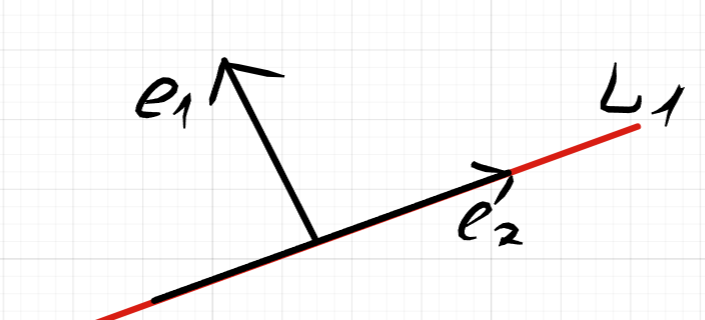
\includegraphics[width = \textwidth]{images/map_form_soglBasis.png}
    \caption{Пример согласованного базиса, так как $L_1 = <\!e_2\!>$}
  \end{subfigure}
  \hfill
  \begin{subfigure}[b]{0.4\textwidth}
    \centering
    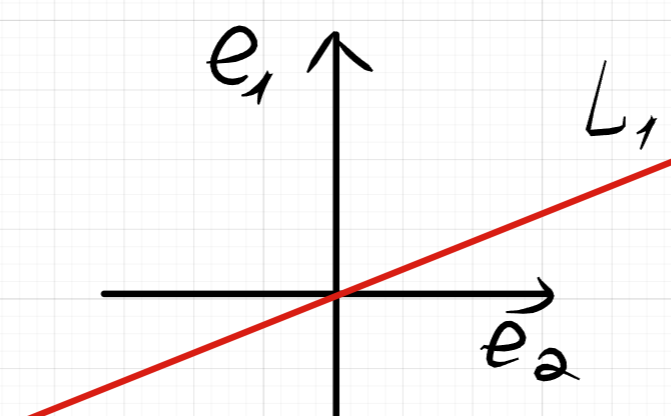
\includegraphics[width = \textwidth]{images/map_form_NesoglBasis.png}
    \caption{Пример несогласованного базиса}
  \end{subfigure}
\end{figure}

\begin{definition}
  \textit{Суммой} подпространств $L_1,L_2, \ldots, L_k$ называется совокупность векторов вида $\bar{u}_1 + \bar{u}_2 + \ldots + \bar{u}_k$, где $\bar{u}_i \in L_i,~ i = 1,\ldots,k.$
\end{definition}


\begin{theorem}
  Для всякой пары подпространств $L_1,\; L_2 \in L$ существует базис пространства $L$, согласованный с подпространствами $L_1,\;L_2$.
\end{theorem}
\begin{Proof}
  Пусть $(\bar{e}_1, \ldots, \bar{e}_k)$ "--- базис $L_1 \cap L_2$.Дополним до базиса $L_1$ и $L_2$:

  $(\bar{e}_1, \ldots, \bar{e}_k, \bar{f}_1, \ldots, \bar{f}_m)$ "--- базис $L_1$.

  $(\bar{e}_1,\ldots, \bar{e}_k, \bar{d}_1, \ldots, \bar{d}_p)$ "--- базис $L_2$.

  Рассмотрим $(\bar{e}_1, \ldots, \bar{e}_k, \bar{f}_1, \ldots, \bar{f}_m,\bar{d}_1, \ldots, \bar{d}_p)$ и докажем, что векторы линейно независимы.
  \begin{gather*}
    \sum_{j = 1}^{k}\lambda_j \, \bar{e}_j + \sum_{j = 1}^{m} \mu_j \, \bar{f}_j + \sum_{j = 1}^{p} \nu_j \, \bar{d}_j = 0 \\
    \underbrace{\sum_{j = 1}^{k}\lambda_j \, \bar{e}_j + \sum_{j = 1}^{m} \mu_j \, \bar{f}_j}_{\in \, L_1} = \underbrace{-\sum_{j = 1}^{p} \nu_j \, \bar{d}_j}_{\in \, L_2} 
  \end{gather*}
  Векторы $(d_1, \ldots, d_p) \notin L_1 \cap L_2 \implies$ равенство возможно только, если все коэффициенты равны нулю, то есть векторы линейно независимы.
\end{Proof}

\begin{corollary}
  $dim\,(L_1 + L_2) = dim\,L_1 + dim\,L_2 - dim\,(L_1 \cap L_2)$  
\end{corollary}

\begin{definition}
  Подпространства $L_1, \ldots, L_k$ называются \textit{линейно независимыми}, если из равенства $\bar{u}_1 + \bar{u}_2 + 
  \ldots + \bar{u}_k = \bar{0},~ \bar{u}_i \in L_i$ следует $\bar{u}_1 = \bar{u}_2 = \ldots = \bar{u}_k = \bar{0}$. 
\end{definition}

\begin{definition}
  Векторное пространство $L$ \textit{разлагается} в прямую сумму подпространств $L_1, \ldots, L_k$, если 
  \begin{enumerate}
    \item $L_1, \ldots, L_k$ "--- линейно независимые
    \item $L_1 + \ldots + L_k = L$
  \end{enumerate}
  Обозначение: $L = L_1 \oplus L_2 \oplus \ldots \oplus L_k$.
\end{definition}
$\forall \bar{v} \in L ~ \bar{v} = \bar{u}_1 + \bar{u}_2 + \ldots + \bar{u}_k,~ \bar{u}_i \in L_i ~ u_i$ называется \textit{проекцией} $v$ на $L_i$.

Напомним, что \textit{линейной} функией называют функцию $\alpha: V \to \Real$, где $V$ "--- векторное пространство (Далее $L,\; V, \; L_i, \; V_i$ "--- векторные пространства), если выполняются следующие условия:
\begin{enumerate}
  \item $\alpha(\bar{x} + \bar{y}) = \alpha(\bar{x}) = \alpha(\bar{y})$
  \item $\alpha(\lambda \bar{x}) = \lambda \alpha(\bar{x})$.
\end{enumerate}
$\forall \, \bar{x},\; \bar{y} \in V$.
\begin{example}
  \textit{След квадратной матрицы} "--- это сумма её диагональных элементов.
  $tr\, A = a_1^1 + a_2^2 + \ldots + a_n^n$

  След квадратной матрицы есть линейная функция, заданная на множестве квадратных матриц. $\alpha(A) = tr\,A , ~ V = M_{m \times n}$.
\end{example}

\begin{definition}
  Линейные функции \textit{образуют} подпространство в пространстве всех функций, заданных на $V$ со значениями $\Real$. 

  Пространство линейных функций, заданных на $V$, называется \textit{сопряженным пространством} по отношению $V$. Обозначение: $V^{\ast}$.
\end{definition}

Пусть $(\bar{e}_1, \ldots, \bar{e}_n)$ "--- базис $V$, а $(\eps_1, \ldots, \eps_n)$ "--- базис $V^{\ast}$.

$\eps_{i} \, (\bar{e}_j) = \delta_{ij} = \begin{cases}
  1&, \text{если } i = j \\
  0&, \text{если } i \neq j.
\end{cases} ~~\text{(символ Кронекера)}$

$\eps_i(\bar{x}) = x_i$.

Напомним также, что \textit{билинейной} функцией (формой) называется функция $\alpha: V \times V \to \Real$, которая линейна по каждому аргументу.

Примером билинейной функции является след: $\alpha(A,B) = tr \, (AB)$.

\begin{definition}
  \textit{Ядром} билинейной функии называется подпространство $Ker\, \alpha = \{\bar{y},~ \alpha(\bar{x}, \bar{y}) = 0,~ \forall \, \bar{x} \in V \}$.
\end{definition}
\begin{definition}
  Функция $\alpha$ называется \textit{невырожденной}, если ядро состоит из нуля ($Ker\, \alpha = 0$).
\end{definition}

Функция $\alpha$ является симметрической, если $\alpha(\bar{x}, \bar{y}) = \alpha(\bar{y}, \bar{x})$.

Функция $\alpha$ является кососимметрической, если $\alpha(\bar{x}, \bar{y}) = -\alpha(\bar{y}, \bar{x})$.

\begin{definition}
  Пусть $\alpha$ симметрическая билинейная функция над полем $K,~ char\, K \neq 2$. Функция $q: V \to K$, которая определяется как $q(\bar{x}) = \alpha(\bar{x}, \bar{x})$, называется \textit{квадратичной} функцией или формой, ассоциированной с функцией $\alpha$
\end{definition}

В координатной форме квадратичную функцию можно записать так:
$$
  q(\bar{x}) = \sum_{i,\, j} a_{ij}\,x_i\, x_j
$$

Симметрическая билинейная функция может восстанавливаться по соответствующей квадратичной функции.
$\alpha(\bar{x},\, \bar{y}) = \frac{1}{2} (q(\bar{x} + \bar{y}) - q(\bar{x}) - q(\bar{y}))$.
\begin{Proof}
  \begin{gather*}
    q(\bar{x} + \bar{y}) = \alpha(\bar{x} + \bar{y},\, \bar{x} + \bar{y}) = \\
    = \alpha(\bar{x}, \, \bar{x}) + \alpha(\bar{y},\, \bar{x}) + \alpha(\bar{x}, \, \bar{y}) + \alpha(\bar{y}, \, \bar{y}) = \\
    = \alpha(\bar{x}, \, \bar{x}) + \alpha(\bar{y}, \, \bar{y}) + 2\alpha(\bar{x}, \, \bar{y}) \implies \\
    2\alpha(\bar{x}, \, \bar{y}) = q(\bar{x} + \bar{y}) - q(\bar{x}) - q(\bar{y})
  \end{gather*}
\end{Proof}

\begin{definition}
  Векторы $\bar{x}$ и $\bar{y}$ называются \textit{ортогональными}, если $\alpha(\bar{x}, \, \bar{y}) = 0$.
\end{definition}

\begin{definition}
  \textit{Ортогональным дополнением} к подпространству $U$ относительно $\alpha$ называется подпространство $U^+ = \{\bar{y}:~ \alpha(\bar{x}, \, \bar{y}) = 0, ~ \forall \, \bar{x} \in U\}$.

  Заметим, что $U^{+} = Ker\; \alpha$.
\end{definition}  

\begin{figure}[H]
  \centering
  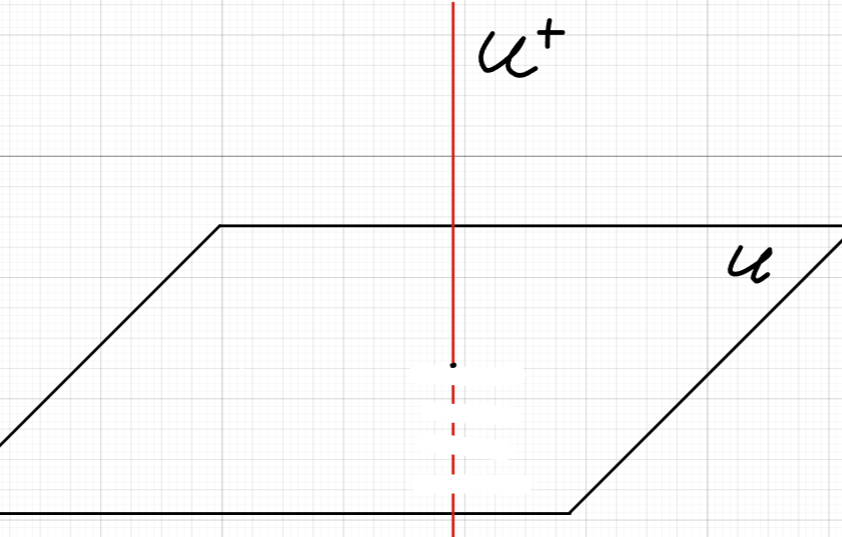
\includegraphics[height = 3cm]{images/map_form_ortog.png}
  \caption{Пример ортогонального дополнения к $U$ относительно скалярного произведения}
\end{figure}

\begin{definition}
  Подпространство $U$ называется \textit{невырожденным} относительно билинейной функции $\alpha$, елси её ограничения на $U$ невырожденно
\end{definition}

\begin{definition}
  Пусть $\alpha$ "--- симметрическая билинейная форма. Базис $(\bar{e}_1, \ldots, \bar{e}_n)$ называется \textit{ортогональным} относительно $\alpha$, если его векторы попарно ортогональны.

\end{definition}
В ортогональном базисе верны следующие утверждения:
\begin{itemize}
  \item[] $\alpha(\bar{x}, \, \bar{y}) = \alpha_1 \, x_1 \, y_1 + \ldots + \alpha_n \, x_n \, y_n$
  \item[] $q(\bar{x}) = \alpha(\bar{x}, \bar{x}) = \alpha_1 \, x_1^2 + \ldots + \alpha_n \, x_n^2$
  \item[] $\alpha(\bar{e}_i, \, \bar{e}_j) = 0$, если $i \neq j$
  \item[] $\alpha_i = \alpha(\bar{e}_i, \, \bar{e}_i)$
\end{itemize}

\begin{theorem}
  \label{theorem: gram_schmidt}
  Пусть $(\bar{e}_1, \bar{e}_2, \ldots, \bar{e}_n)$ "--- базис $V$, $A$ "--- матрица функции $\alpha$ в этом базисе, $A_k$ "--- матрица функции $\alpha$ на подпространстве $V_k = <\!\bar{e}_1, \ldots, \bar{e}_k \!>, ~ k \leq n$ и $\delta_k = det\,A_k$.

  Если все угловые миноры ($\delta_1, \ldots, \delta_n)$ отличны от нуля, то \textbf{сущестует} единственный ортогональный базис $(\bar{f}_1, \ldots, \bar{f}_n)$ удовлетворяющий условию $\bar{f}_k \in \bar{e}_k + V_{k - 1},~ k = 1, \ldots, n$.

  При этом $q(\bar{f}_k) = \alpha(\bar{f}_k, \, \bar{f}_k) = \frac{\delta_k}{\delta_{k - 1}}$.
\end{theorem}

\begin{definition}
  Процесс построения ортогонального базиса называется процессом \textit{ортогонализации Грама"=Шмидта}.
\end{definition}
\begin{example}
  Процесс ортогонализации Грама"=Шмидта:
  \begin{figure}[H]
    \centering
    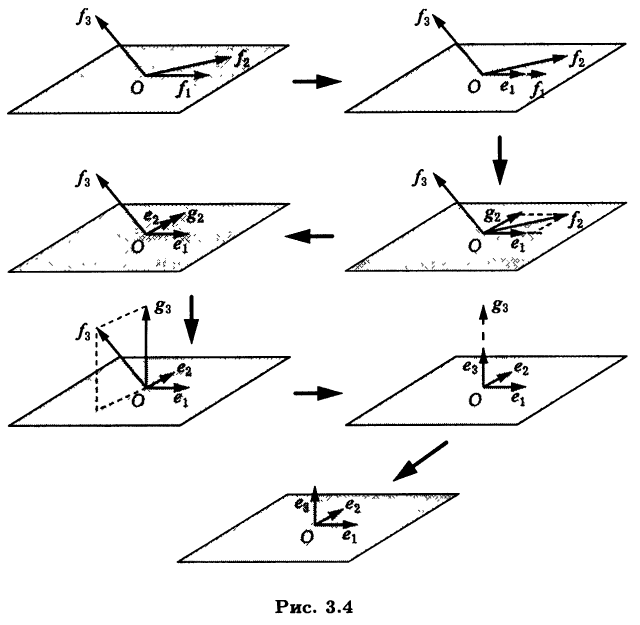
\includegraphics[width= \textwidth]{images/map_form_gram-shmidt.png}
  \end{figure}
\end{example}
Построение ортонормированного базиса:

$(\bar{e}_1, \ldots, \bar{e}_n)$ "--- базис $\rightarrow ~ (\bar{f}_1, \ldots, \bar{f}_n)$ "--- ортогональный базис ($\bar{f}_i \; \bot \; \bar{f}_j, ~ \alpha(\bar{f}_i, \, \bar{f}_j) = 0$ при $i \neq j$) $\rightarrow ~ (\bar{d}_1, \ldots, \bar{d}_n)$ "--- ортонормированный базис ($\mathopen| \bar{d}_i \mathclose| = 1$).

\begin{definition}
  Вещественная квадратичная форма $q$ называется \textit{положительно определенной}, если $q(\bar{x}) > 0,~ \bar{x} \neq \bar{0}$

  Вещественная симметрическая билинейная форма назыается \textit{положительно определенной}, если соответствующая ей квадратичная форма положительно определена.
\end{definition}
\begin{theorem}[Критерий Сильвестра]
  Вещественная квадратичная функция является \textbf{положительно определённой} тогда и только тогда, когда все угловые миноры её матрицы \textbf{положительны}.
\end{theorem}
\subsection*{Канонический вид квадратичных форм}

Если квадратичная функция $q: V \to \Complex$ определена на поле комплексных чисел, то путём нормировки базисных векторов квадратичную форму можно привести к виду 
$$q(\bar{x}) = x_1^2 + \ldots + x_r^2,$$ где $r$ "--- ранг квадратичной формы.

В случае же, когда квадратичная форма $q: V \to \Real$ определена на поле вещественных чисел, то форму можно привести к виду 
\begin{equation}
  \label{eq:quad_real}
  q(\bar{x}) = x_1^2 + x_2^2 + \ldots + x_k^2 - x_{k + 1}^2 - x_{k + 2}^2 - \ldots - x_{k + \ell}^2,
\end{equation}
где $k + \ell$ "--- ранг формы.

Число $k$ в нормальном виде квадратичной формы \ref{eq:quad_real} есть \textit{максимальная размерность подпространства}, на котором функция $q$ положительно определена.

\begin{theorem}[Закон инерции]
  Числа $k$ и $\ell$ в нормальном виде \ref{eq:quad_real} вещественной квадратичной функции не зависят от выбора базиса, в котором эта функция имеет нормальный вид.

  Пара $(k, \, \ell)$ называется \textbf{сигнатурой} квадратичной функции.
\end{theorem}

\subsection*{Евклидово пространство}

\begin{definition}
  \textit{Евклидовым векторным пространством} называется действительное векторное пространство с фиксированным положительно определенной симметрической билинейной функцией. Эта функция называется \textit{скалярным произведением}.
\end{definition}

\begin{definition}
  \textit{Матрицей Грама} (в евклидовом пространстве) называется $$
  G(\bar{e}_1, \ldots, \bar{e}_n) = \begin{pmatrix}
    (\bar{e}_1,\, \bar{e}_1) & (\bar{e}_1,\, \bar{e}_2) & \ldots & (\bar{e}_1,\, \bar{e}_n) \\
    (\bar{e}_2,\, \bar{e}_1) & (\bar{e}_2,\, \bar{e}_2) & \ldots & (\bar{e}_2,\, \bar{e}_n) \\
    \vdots & \vdots && \vdots \\
    (\bar{e}_n,\, \bar{e}_1) & (\bar{e}_n,\, \bar{e}_2) & \ldots & (\bar{e}_n,\, \bar{e}_n)
  \end{pmatrix},
  $$
  где $(\bar{e}_i,\, \bar{e}_j)$ "--- скалярное произведение. Так как функция симметрическая, то матрица симметрична относительно главной диагонали.
\end{definition}
(Не было на лекциях) Матрица Грама обладают следующими свойствами:
\begin{itemize}
  \item[] Определитель матрицы Грама системы $n$ векторов равен квадрату объёма 
  $n$"=мерного параллелепипеда, натянутого на эти векторы. Из этого следует, что в случае трёхмерного пространства определитель Грама трёх векторов равен квадрату их смешанного произведения.
  \item[] Система векторов $v_1, \ldots, v_n$ линейно зависима тогда и только тогда, когда определитель матрицы Грама этой системы равен нулю.
\end{itemize}

Пусть $L = U \oplus U^+ \implies \underbrace{\bar{x}}_{\in \, L} = \underbrace{\bar{y}}_{\in \, U} + \underbrace{\bar{z}}_{\in\, U_+}$, где $\bar{y}$ "--- ортогональная \textit{проекция} $\bar{x}$ на $U$, $\bar{z}$ "--- ортогональная \textit{составляющая} $\bar{x}$ относительно $U$.

Пусть $(\bar{e}_1, \ldots, \bar{e}_k)$ "--- ортогональный базис $U$.

Зная $\bar{x}$,
\textbf{Как найти проекцию и составляющую?}
\begin{gather*}
  \bar{x} = \lambda_1 \, \bar{e}_1 + \lambda_2 \, \bar{e}_2 + \ldots + \lambda_k \, \bar{e}_k + \bar{z} ~~/ \text{ Скалярно умножаем на } \bar{e}_1 \\
  (\bar{x}, \, \bar{e}_1) = \lambda_1(\bar{e}_1,\, \bar{e}_1) + \lambda_2\underbrace{(\bar{e}_1, \, \bar{e}_2)}_{ = \, 0} + \ldots + \lambda_k \underbrace{(\bar{e}_k, \, \bar{e}_1)}_{ = \, 0} + \underbrace{(\bar{z}, \, \bar{e}_1)}_{= \, 0} \\
  \lambda_1 = \frac{(\bar{x}, \, \bar{e}_1)}{\bar{e}_1^2} \\
  \text{Проделывая аналогочные действия для всех } i = 1, \ldots, k  \text{, получим:}\\
  \lambda_i = \frac{(\bar{x}, \bar{e}_i)}{\bar{e}_i^2} \\
  \implies \bar{x} = \underbrace{\sum_{i = 1}^{k} \frac{(\bar{x}, \, \bar{e}_i)}{(\bar{e}_i, \, \bar{e}_i)} \cdot \bar{e}_i}_{y} + \bar{z} \implies \bar{z} = \bar{x} - \bar{y}.  
\end{gather*}

По теореме \ref{theorem: gram_schmidt} мы знаем, когда существует ортогональный базис, но
\textbf{Как построить ортогональный базис?}

Пусть $(\bar{e}_1, \ldots, \bar{e}_n)$ "--- произвольный базис. Построим ортогональный базис $(\bar{f}_1, \ldots, \bar{f}_n)$.

$\bar{f}_1 = \bar{e}_1$

$\bar{e}_2 = \lambda_1 \, \bar{e}_1 + \bar{f}_2,$ где $\bar{f}_2$ "--- ортогональная составляющая. Умножаем выражение скалярно на $\bar{f}_1 = \bar{e}_1$ 

$(\bar{e}_2, \, \bar{f}_1) = \lambda_1 \, (\bar{e}_1, \, \bar{f}_1) + \underbrace{(\bar{f}_2,\, \bar{f}_1)}_{\substack{= \, 0, \\ \text{так как } \bar{f}_2 \; \bot \; \bar{f}_1}}$

$\lambda_1 = \frac{(\bar{e}_2, \, \bar{f}_1)}{(\bar{f}_1, \bar{f}_1)} \implies \bar{f}_2 = \bar{e}_2 - \lambda_1 \, \bar{e}_1$

$\bar{e}_3 = \lambda \, \bar{f}_1 + \mu \, \bar{f}_2 + \bar{f}_3$

Скалярно умножаем на $f_1$: $\lambda = \frac{(\bar{e}_3, \, \bar{f}_1)}{(\bar{f}_1, \, \bar{f}_1)}$

Скалярно умножаем на $f_2$: $\mu = \frac{(\bar{e}_3, \, \bar{f}_2)}{(\bar{f}_2, \, \bar{f}_2)}$

$\implies \bar{f}_3 = \bar{e}_3 - \lambda \, \bar{f}_1 - \mu \, \bar{f}_2$

Следовательно $\bar{f}_i = \bar{e}_i - \sum\limits_{k = 1}^{i - 1} \frac{(\bar{e}_i, \, \bar{f}_k)}{(\bar{f}_k, \, \bar{f}_ k)} \cdot \bar{f}_k, ~ i = 1, \ldots, n$

\begin{definition}
  Евклидовые векторные пространства $V, \, U$ называются изоморфными, если существует биективное отображение $f: V \to U$ являющаяся изоморфизмом и выполняется равенство $(f(\bar{a}), \, f(\bar{b})) = (\bar{a}, \bar{b}),~ \forall \, \bar{a}, \, \bar{b} \in V.$
\end{definition}

\begin{theorem}
  Любые два евклидовых векторных пространства одинаковой размерности изоморфны.
\end{theorem}
\begin{Proof}
  Пусть $dim \, V = dim \, U = n,~ U,\, V$ "--- векторные пространства,

  $(\bar{v}_1, \ldots, \bar{v}_n), \, (\bar{u}_1, \ldots, \bar{u}_n)$ "--- ортонормированные базисы $V$ и $U$ соответственно.

  Построим отображение
  $f: V \to U, ~f(\bar{v}_i) = \bar{u}_i,~$ а значит $(f(\bar{v}_i), \, f(\bar{v}_k)) = (\bar{u}_i, \, \bar{u}_k) = \delta_{ik} = (\bar{v}_i, \, \bar{v}_k)$.

  Следовательно $V$ и $U$ изоморфны.
\end{Proof}

\subsection*{Линейный оператор}
\begin{definition}
  \textit{Линейным оператором} или \textit{линейным преобразованием} векторного пространства $L$ называется линейное отображение в себя $A: L \to L$.
  
  Выполняются следующие условия:
  \begin{enumerate}
    \item $A(\bar{x} + \bar{y}) = A\, \bar{x} + A \, \bar{y}$
    \item $A(\lambda\bar{x}) = \lambda A\, \bar{x}$
  \end{enumerate}
\end{definition}

Пусть $(\bar{e}_1, \ldots, \bar{e}_n)$ "--- базис $L$,
\begin{gather*}
  A(\bar{e}_1) = a_1^1\bar{e}_1 + a_1^2\bar{e}_2 + \ldots + a_1^n\bar{e}_n \\
  \vdots \\
  A(\bar{e}_n) = a_n^1\bar{e}_1 + a_n^2\bar{e}_2 + \ldots + a_n^n \bar{e}_n \\
  \underbrace{(A\, \bar{e}_1, \ldots, A\, \bar{e}_n)}_{\text{матрица"=строка}} = \underbrace{(\bar{e}_1, \ldots, \bar{e}_n)}_{\text{матрица"=строка}} \cdot \begin{pmatrix}
    a_1^1 & \cdots & a_n^1 \\
    \vdots & \ddots & \vdots \\
    a_1^n & \cdots & a_n^n
  \end{pmatrix} \\
  A\, \bar{e}_i = \sum_{k = 1}^n \, a_i^k \bar{e}_k, ~ k = 1, \ldots, n 
\end{gather*}
\begin{definition}
  Матрица $\begin{pmatrix}
    a_1^1 & \cdots & a_n^1 \\
    \vdots & \ddots & \vdots \\
    a_1^n & \cdots & a_n^n
  \end{pmatrix}$ называется \textit{матрицей линейного оператора } $A$.
\end{definition}

Рассмотрим переход от базиса $(\bar{e}_1, \ldots, \bar{e}_n)$ к $(\bar{e}_1', \ldots, \bar{e}_n')$:

$(\bar{e}_1, \ldots, \bar{e}_n) = (\bar{e}_1', \ldots, \bar{e}_n') \cdot C$, где $C$ "--- матрица перехода от $(\bar{e}_i)$ к $(\bar{e}_i')$.

$(A\, \bar{e}_1', \ldots, A\, \bar{e}_n') = (\bar{e}_1', \ldots, \bar{e}_n') \cdot A'$, где $A'$ "--- матрица линейного оператора в базисе $(\bar{e}_i')$. Аналогично для базиса $(\bar{e}_1, \ldots, \bar{e}_n)$.

$(A\, \bar{e}_1', \ldots, A\, \bar{e}_n') = (A\, \bar{e}_1, \ldots, A\, \bar{e}_n) \cdot C = (\bar{e}_1, \ldots, \bar{e}_n) \cdot A\, C \implies$

$(\bar{e}_1', \ldots, \bar{e}_n') \cdot A' = (\bar{e}_1, \ldots, \bar{e}_n) \cdot A\, C \implies$

$\underline{A' = C^{-1} \cdot A \cdot C}$

\begin{definition}
  Подпространство $\mathcal{U} \in L$ называется \textit{инвариантным} относительно оператора $A$, если $A\,(\mathcal{U}) \in \mathcal{U}$.

  То есть $\bar{x} \in \mathcal{U} \implies A\, \bar{x} \in \mathcal{U}$.
\end{definition}

Если $\mathcal{U} = <\! \bar{e}_1, \ldots, \bar{e}_k \!>$, а $L =  <\! \bar{e}_1, \ldots, \bar{e}_k, \bar{e}_{k + 1}, \ldots, \bar{e}_n\!>$ (а это всегда можно сделать), то матрица оператора $A$ в этом базисе имеет вид:
$$
A = \begin{pmatrix}
  B & D\\
  0 & C
\end{pmatrix},
$$
где $B$ "--- матрица оператора $A_\mathcal{U}$ в базисе $<\! \bar{e}_1, \ldots, \bar{e}_k \!>$, $C$ "--- квадратная матрица порядка $n - k$ и $D$ "--- какая"=то матрица размера $k \times (n - k)$. Верно и обратное.

Если же пространство $L$ можно разложить на сумму двух инвариантных подпространств $\mathcal{U}_1$ и $\mathcal{U}_2$: $L = \mathcal{U}_1 \oplus \mathcal{U}_2$, то матрица линейного оператора имеет вид:
$$
A = \begin{pmatrix}
  B & 0 \\
  0 & C
\end{pmatrix},
$$
где $B$ "--- матрица оператора $A_{\mathcal{U}_1}$, $C$ "--- матрица оператора $A_{\mathcal{U}_2}$.

\subsection*{Собственные векторы}
\begin{definition}
  Пусть $A: L \to L$ "--- линейный оператор. Вектор $\bar{x} \neq 0$ называется \textit{собственным} вектором оператора $A$, если $A\, \bar{x} = \lambda \bar{x}, ~ \lambda \in \Real$, где число $\lambda$ "--- \textit{собственное значение} оператора $A$, отвечающие собственному вектору $\bar{x}$.
\end{definition}

Если $(\bar{e}_1, \ldots, \bar{e}_n)$ "--- базис из собственных векторов, то матрица линейного оператора выглядит следующим образом:
$$
  A = \begin{pmatrix}
    \lambda_1 & 0 & \cdots & 0 \\
    0 & \lambda_2 & \cdots & 0 \\
    \vdots & \vdots && \vdots \\
    0 & 0 & \cdots & \lambda_n
  \end{pmatrix}
$$
\begin{theorem}
  Для существования $\bar{x}$ и $\lambda$ необходимо и достаточно $det\, (A - \lambda E) = 0$, где $A$ "--- матрица линейного оператора, $E$ "--- единичная матрица.
\end{theorem}
\begin{Proof}
  $A\, \bar{x} = \lambda \bar{x}$

  $A\, \bar{x} - \lambda \bar{x} = 0$

  $(A - \lambda E)\bar{x} = 0$ Записав в координатном виде это равенство, получим однородную систему линейных уравнений.


  У этой системы есть ненулевое решение $\Leftrightarrow det\, (A - \lambda E) = 0$.
\end{Proof}

\begin{definition}
  Многочлен $f_A(t) = det\, (A - tE)$ называется \textit{характеристическим} многочленом оператора $A$.
\end{definition}

\begin{theorem}
  Характеристический многочлен не зависит от выбора матрицы линейного оператора, то есть $det\, (A_1 - tE) = \det (A_2 - tE)$, где $A_1, \, A_2$ "--- матрицы линейного оператора $A$ в базисе $(\bar{e}_i)$ и $(\bar{e}_j)$.
\end{theorem}
\begin{Proof}
  Пусть $C$ "--- матрица перехода из $\bar{e}_i$ в $\bar{e}_i'$, то есть $\bar{e}_i' = \sum\limits_{j = 1}^n \, C_i^j\; \bar{e}_j$

  $A_2 = C^{-1} \cdot A_1 \cdot C$

  $\det(A_2 - tE) = \det(C^{-1}\, A_1 \, C - tE) = \det(C^{-1}\, A_1\, C - t\, C^{-1}\, C) = $

  $= \det C^{-1}(A_1 - tE)C = \det C^{-1} \cdot \det (A_1 - tE) \cdot \det C = $

  $= det(\underbrace{C^{-1} \cdot C}_{E}) \cdot \det(A_1 - tE) = \det(A_1 - tE)$.  
\end{Proof}

\begin{theorem}
  Собственное значение оператора $A$ "--- это корень его характеристического многочлена.
\end{theorem}

\begin{theorem}
  Любой линейный оператор в комплексном линейном пространстве имеет собственный вектор
\end{theorem}

\begin{theorem}
  Пусть $A: L \to L,~ L \subset \Real$, тогда существует одномерное или двумерное инвариантное подпространство.

  (Для любого линейного оператора над полем вещественных чисел существует одномерное или двумерное инвариантное подпространство).
\end{theorem}

При заданном значении $\lambda$ собственные векторы находятся из системы однородных линейных уравнений
$$
  (A - \lambda E)X = 0,
$$
где $X$ обозначает столбец координат неизвестного вектора. Вместе с нулевым вектором они составляют подпространство
$$
  V_\lambda(A) = \ker(A - \lambda E),
$$
называемое \textit{собственным подпространством} оператора $A$, отвечающим собственному значению $\lambda$. Его размерность равна $n - \operatorname{rk}(A - \lambda E)$.

\begin{theorem}[о собственных подпространствах, отвечающих различным собственным значениям оператора]
  Собственные подпространства, отвечающие различным собственным значениям $\lambda_1, \ldots, \lambda_k$ оператора $A$, линейно независимы.
\end{theorem}

\begin{theorem}[Необходимое и достаточное условие существования базиса из собственных векторов линейного оператора]
  Для существования базиса из собственных векторов линейного оператора $A$ необходимо и достаточно, чтобы выполнялись следующие условия:
  \begin{enumerate}
    \item Характеристический многочлен $f_A(t)$ разлагается на линейные множители
    \item Размерность каждого собственного подпространства равна кратности соответствующего корня многочлена $f_A(t)$.
  \end{enumerate}
\end{theorem}

\subsection*{Линейные операторы и билинейные функции в евклидовом пространстве}
\begin{definition}
  Пусть $A$ "--- линейный оператор. Тогда билинейная функция оператора $A$ опеределяется как
  $$
    \varphi_A(\bar{x}, \, \bar{y}) = (\bar{x}, \, A\, \bar{y}) 
  $$
  Если $\varphi_A(\bar{x}, \, \bar{y}) = \varphi_A(\bar{y},\, \bar{x})$, то $A$ называют \textit{симметрическим} или \textit{самосопряженным} оператором.
\end{definition}

\begin{theorem}
  В ортонормированном базисе матрицы $\varphi_A$ и $A$ совпадают.
\end{theorem}
\begin{Proof}
  Пусть $(\bar{e}_i)$ "--- ортонормированный базис.

  $\varphi_A(\bar{e}_i, \bar{e}_k) = \bar{e}_i A\, \bar{e}_k = \bar{e}_i \sum\limits_{j = 1}^n \, a_k^j \, \bar{e}_j = \sum\limits_{j = 1}^n \, a_k^j \, \bar{e}_j \cdot \bar{e}_i = \sum\limits_{j = 1}^n \, a_k^j \, \delta_j^i = a_k^i$, так как $\delta_j^i = 1 \Leftrightarrow i = j$.
\end{Proof}

\begin{theorem}
  Пусть $V \subset E, ~ AV \subset V$. Тогда $AV^{\bot} \subset V^{\bot}$. То есть, если подпространство $V$ инвариантно, то и его ортогональное дополнение $V^{\bot}$ инвариантно.
\end{theorem}
\begin{Proof}
  $(\bar{x}, \, \bar{y}) = \bar{0},~ \bar{x} \in V, ~ \bar{y} \in V^{\bot}$

  $\bar{x} A\, \bar{y} = \varphi_A(\bar{x}, \, \bar{y}) = \varphi_A(\bar{y},\, \bar{x}) = \bar{y} A\, \bar{x} = \bar{0}$

  $\underbrace{\bar{x}}_{\in \, V} A\, \bar{y} = \bar{0} \implies A\, \bar{y} \in \, V^{\bot} \implies AV^{\bot} \subset V^{\bot} \implies$
  
  $V^{\bot}$ "--- инвариантное подпространство. 
\end{Proof}

\begin{theorem}
  Для самосопряженного оператора существует ортонормированный базис, состоящий из собственных векторов.
\end{theorem}

\begin{theorem}
  Пусть $\varphi$ "--- симметрическая билинейная форма. Тогда существует такой ортонормированный базис, в котором форма имеет канонический вид:
  $$
    \varphi(\bar{x}, \, \bar{y}) = \lambda_1 x_1 y_1 + \lambda_2 x_2 y_2 + \ldots + \lambda_n x_n y_n
  $$
\end{theorem}

\section*{Фигуры второго порядка на плоскости и в пространстве}
\begin{definition}
  В аффиной системе координат общее уравнение линии второго порядка имеет вид:  
  \begin{equation}
    \label{eq:fig_common}
    F(x,\, y) = \underbrace{a_{11}x^2 + a_{22}y^2}_{\text{квадратичная часть}} + 
  \underbrace{2a_{12}xy + 2a_{10}x + 2a_{20}y}_{\text{линейная часть}} + a_{00} = 0,
  \end{equation}
  в котором коэффициенты "--- любые действительные числа, причем $a_{11},\, a_{12}, \, a_{22}$ не равны одновременно нулю.
\end{definition}

Уравнение \ref{eq:fig_common} можно записать в виде:
$$
  F(x, \, y) = \begin{pmatrix} x & y \end{pmatrix} \; \begin{pmatrix}
    a_{11} & a_{12} \\
    a_{21} & a_{22}
  \end{pmatrix} \; \begin{pmatrix} x \\ y \end{pmatrix} + 2 \begin{pmatrix} a_{10} & a_{20} \end{pmatrix} \begin{pmatrix} x \\ y \end{pmatrix} + a_{00} = 0
$$

\begin{lemma}
  Подходящим поворотом осей координат можно добиться того, что $a_{12}'= 0$, где штрих означает соответствующий коэффициент уравнения кривой второго порядка в новой системе координат.
\end{lemma}
\begin{Proof}
  Рассмотрим поворот: 
  $$
  \begin{pmatrix} x \\ y \end{pmatrix} = 
  \begin{pmatrix}
    \cos \varphi & -\sin \varphi \\
    \sin \varphi & \cos \varphi
  \end{pmatrix} \begin{pmatrix} x' \\ y' \end{pmatrix}
  $$
  Тогда 
  \begin{gather*} F(x', \, y') = a_{11}(x'\, \cos \varphi - y' \, \sin \varphi)^2 + a_{22} (x' \, \sin \varphi + y'\, \cos \varphi)^2 + \\ + 2a_{12}(x' \, \cos \varphi - y' \, \sin \varphi)(x' \, \sin \varphi + y'\, \cos \varphi)+
  2a_{10}(x'\, \cos \varphi - y' \, \sin \varphi) + \\ + 2a_{20}(x' \, \sin \varphi + y' \, \cos \varphi) + a_{00} = 0 
  \end{gather*}
  Коэффициент при $2x'\, y'$, то есть $a_{12}'$ равен
  \begin{gather*}
    a_{12}' = -a_{11}\cos \varphi \sin \varphi + a_{12}(\cos^2 \varphi - \sin^2 \varphi) + a_{22}\cos \varphi \sin \varphi  = 0 \\
    a_{12}\cos 2\varphi = \frac{1}{2} \sin 2\varphi (a_{11} - a_{22}) \\
    \operatorname{tg} 2 \varphi = \frac{2a_{12}}{a_{11} - a_{22}} 
  \end{gather*}
\end{Proof}
Выполнив поворот оси на угол $\varphi$, многочлен $F$ примет вид:
\begin{equation}
  \label{eq:fig_del12}
  F'(x', \, y') = \lambda_1 x'^{\, 2} + \lambda_2 y'^{\, 2} + 2b_1x' + 2b_2y' + b_0 = 0
\end{equation}
\begin{lemma}
  Многочлен вида \ref{eq:fig_del12} параллельным переносом приводится к одному из следующих видов:
  \begin{enumerate}
    \item \begin{equation}
      \label{eq:lemma_1}
      F'' = \lambda_1(x'')^2 + \lambda_2(y'')^2 + \tau, ~ (\lambda_1,\, \lambda_2 \neq 0)
    \end{equation}
    \item \begin{equation}
      \label{eq:lemma_2}
      F'' = \lambda_2(y'')^2 + 2b_1x'', ~ (\lambda_2, \, b_1 \neq 0)
    \end{equation}
      \item \begin{equation}
        \label{eq:lemma_3}
        F'' = \lambda_2(y'')^2 + \tau, ~ (\lambda_2 \neq 0)
      \end{equation}
  \end{enumerate}
\end{lemma}
\begin{Proof}
  \begin{enumerate}
    \item $\lambda_1, \, \lambda_2 \neq 0$
    \begin{gather*}
      F'(x', \, y') = \lambda_1 x'^{\, 2} + \lambda_2 y'^{\, 2} + 2b_1x' + 2b_2y' + b_0 =\\
      =\lambda_1 \Bigl(\underbrace{x' + \frac{b_1}{\lambda_1}}_{x''}\Bigr)^2 + \lambda_2\Bigl(\underbrace{y' + \frac{b_2}{\lambda_2}}_{y''}\Bigr)^2 + \Bigl(\underbrace{b_0 - \frac{b_1^2}{\lambda_1} - \frac{b_2^2}{\lambda_2}}_{\tau}\Bigr) = \\
      = \lambda_1(x'')^2 + \lambda_2(y'')^2 + \tau,
    \end{gather*}
  \end{enumerate}
  \item $\lambda_1 = 0, \; \lambda_2 \neq 0$ (если наоборот, то поменяем координаты местами). Возможны два случая:
  \begin{enumerate}
    \item если $b_1 \neq 0$, то 
    \begin{gather*}
      F'(x', \, y') = \lambda_2 y'^{\, 2} + 2b_1x' + 2b_2y' + b_0 =\\
      = \lambda_2\Bigl(y' + \frac{b_2}{\lambda_2} \Bigr)^2 + 2b_1x' + \Bigl(b_0 - \frac{b_2^2}{\lambda_2}\Bigr) = \\
      = \lambda_2\Bigl(\underbrace{y' + \frac{b_2}{\lambda_2}}_{y''} \Bigr)^2 + 2b_1\Bigl(\underbrace{x' + \frac{1}{2b_1}\bigl(b_0 - \frac{b_2^2}{\lambda_2}\bigr)}_{x''}\Bigr) = \\
      = \lambda_2(y'')^2 + 2b_1x''
    \end{gather*}
    \item если $b_1 = 0$, то
    \begin{gather*}
      F'(x', \, y') = \lambda_2 y'^{\, 2} + b_2y' + b_0 = \\
      = \lambda_2\Bigl(\underbrace{y' + \frac{b_2}{\lambda_2}}_{y''}\Bigr)^2 + \Bigl(\underbrace{b_0 - \frac{b_2^2}{\lambda_2}}_{\tau}\Bigr) = \\
      = \lambda_2(y'')^2 + \tau
    \end{gather*}
  \end{enumerate}
\end{Proof}

\begin{theorem}
  \label{theorem:second}
  Для любой кривой второго порядка существует прямоугольная система координат, в которой она имеет один из следующих видов (называемых каноническими уравнениями):
  \begin{enumerate}
    \item $\frac{x^2}{a^2} + \frac{y^2}{b^2} = 1, ~(a \geq b > 0),$ эллипс 
    \item  $\frac{x^2}{a^2} + \frac{y^2}{b^2} = -1, ~(a \geq b > 0),$ мнимый эллипс 
    \item  $\frac{x^2}{a^2} - \frac{y^2}{b^2} = 1, ~(a \geq b > 0),$ гипербола
    \item  $\frac{x^2}{a^2} - \frac{y^2}{b^2} = 0, ~(a \geq b > 0),$ пара пересекающихся прямых
    \item $\frac{x^2}{a^2} + \frac{y^2}{b^2} = 0, ~(a \geq b > 0),$ пара пересекающихся мнимых прямых 
    \item $y^2 = 2px, ~ (p > 0),$ парабола
    \item $y^2 - a^2 = 0, ~ (a > 0),$ пара параллельных прямых
    \item $y^2 + a^2 = 0, ~ (a > 0),$ пара мнимых параллельных прямых
    \item $y^2 = 0$ пара совпадающих прямых
  \end{enumerate}
\end{theorem}

Рассмотрим различные равенства \ref{eq:lemma_1}--\ref{eq:lemma_3}:
\begin{enumerate}
  \item $F'' = \lambda_1(x'')^2 + \lambda_2(y'')^2 + \tau, ~ (\lambda_1,\, \lambda_2 \neq 0)$
  \begin{enumerate}[label = \alph*)]
    \item $\lambda_1, \, \lambda_2$ "--- одного знака, $\tau$ "--- противоположного. Получаем уравнение эллипса.
    \item $\lambda_1, \, \lambda_2, \, \tau$ "--- одного знака. Получаем уравнение мнимого эллипса.
    \item $\lambda_1, \, \lambda_2$ "--- одного знака, $\tau = 0$. Пара пересекающихся мнимых прямых.
    \item $\lambda_1, \, \lambda_2$ "--- разных знаков, $\tau \neq 0$. Гипербола
    \item $\lambda_1, \, \lambda_2$ "--- разных знаков, $\tau = 0$. Пара пересекающихся прямых.
  \end{enumerate}
  \item $F'' = \lambda_2(y'')^2 + 2b_1x'', ~ (\lambda_2, \, b_1 \neq 0)$. Парабола
  \item $ F'' = \lambda_2(y'')^2 + \tau, ~ (\lambda_2 \neq 0)$
  \begin{enumerate}[label = \alph*)]
    \item $\tau < 0$. Пара параллельных прямых.
    \item $\tau > 0$. Пара мнимых параллельных прямых.
    \item $\tau = 0$. Пара совпадающих прямых.
  \end{enumerate}
\end{enumerate}

\subsection*{Эллипс}
Эллипсом по теореме \ref{theorem:second} была названа линия, которая в некторой прямоугольной системе координат определяется каноническим уравнением:
\begin{equation}
  \label{eq:ellipse}
  \frac{x^2}{a^2} + \frac{y^2}{b^2} = 1
\end{equation}
Из уравнения \ref{eq:ellipse} следует, что для всех точек эллипса $\mathopen|x\mathclose| \leq a$ и $\mathopen|y\mathclose| \leq b$
\begin{figure}[H]
  \centering
  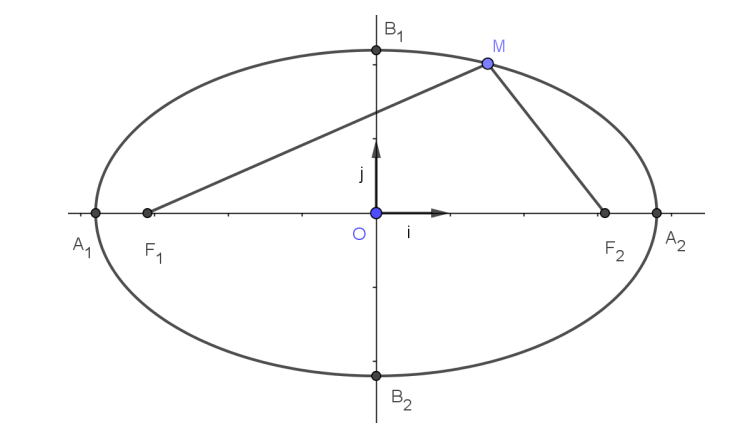
\includegraphics[width = \textwidth]{images/second_ellipse.png}
  \caption{Эллипс. $OA_2 = OA_1 = a, ~ OB_1 = OB_2 = b$}
  \label{fig:ellipse} 
\end{figure}

Точки, имеющие координаты $(a,\, 0), \, (a,\, 0), \, (0,\, b), \, (0,\, -b)$ называются \textit{вершинами} эллипса.

С эллипсом связаны две замечательные точки, называемые его \textit{фокусом} (на рисунке \ref{fig:ellipse} отмечены точками $F_1$ и $F_2$). Пусть по определению 
$$
  c^2 = a^2 - b^2
$$
и $c \geq 0$. Тогда точки $F_1$ и $F_2$ имеют координаты $(-c,\, 0)$ и $(c, \, )$ соответственно. Расстояние между фокусами называется \textit{фокальным расстоянием}.

Если $M$ "--- точка эллипса, то отрезки $F_1M$ и $F_2M$ называются \textit{фокальными радиусами} точки $M$. Их длины также называют фокальными радиусами точки $M$. 

Оказывается для того чтобы точка лежала на эллипсе, необходимо и достаточно, чтобы сумма ее расстояний до фокусов равнялась $2a$. 

\begin{Proof}
  Пусть сумма расстояний до фокусов равняется $2a$. Фокальные радиусы точки $M(x,\, y)$ эллипса равны:
  $$
    F_1M = \sqrt{(x + c)^2 + y^2}, ~~ F_2M = \sqrt{(x - c)^2 + y^2}.
  $$
  и $F_1M + F_2M = 2a$. Запишем это выражение в виде:
  $$
    \sqrt{(x + c)^2 + y^2} = 2a - \sqrt{(x - c)^2 + y^2}.
  $$
  Возводя его в квадрат и приводя подобные члены, получим:
  $$
    a\sqrt{(x - c)^2 + y^2} = a^2 - xc.
  $$
  Снова возводя в квадрат, после преобразований получим:
  $$
    \frac{x^2}{a^2} + \frac{y^2}{b^2} = 1,
  $$
  где $b^2  = a^2 - c^2$. Таким образом, $M$ удовлетворяет уравнению \ref{eq:ellipse}.

  Пусть точка $M$ удовлетворяет уравению \ref{eq:ellipse}. Тогда $F_1M = \sqrt{(a + \frac{c}{a}x)^2} = \mathopen|a + \frac{c}{a}x$, $F_2M = \sqrt{(a - \frac{c}{a}x)^2} = \mathopen|a - \frac{c}{a}x\mathclose|$. 

  Так как $\mathopen|x\mathclose| \leq a$, и так как $0 < e = \frac{c}{a} < 1$, то поэтому $a + \frac{c}{a}x > 0, ~ a - \frac{c}{a}x > 0$, поэтому $$
    F_1M = a - \frac{c}{a}x, ~~ F_2M = a + \frac{c}{a}x.
  $$
  Следовательно, $F_1M + F_2M = 2a$.
\end{Proof}

Учитывая это, можно дать определение эллипса:
\begin{definition}
  \textit{Эллипсом} называется множество всех точек плоскости, сумма расстояний каждой из которых до данных точек $F_1$ и $F_2$ равна длине данного отрезка $PQ$, причем $PQ > F_1F_2$.
\end{definition}

Если точки $F_1$ и $F_2$ совпадают, то эллипс является окружностью радиуса $a$. В этом случае фокусы эллипса совпадают с центром окружности. Таким образом, \textit{окружность есть частный случай эллипса}.

Эллипс имеет один центр симметрии и две оси симметрии. Центр симметрии совпадает с серединой фокального отрезка. Прямая, проходящая через фокусы, называется \textit{первой} или \textit{фокальной} осью симметрии, а перпендикулярная к ней ось "--- второй осью симметрии.

Отрезки $2a \, (A_1A_2)$ и $2b \, (B_1B_2)$ называются \textit{большой} и \textit{малой осями} эллипса а $a$ и $b$ "--- \textit{большой} и \textit{малой полуосями} эллипса.

Отношение
$$
  e = \frac{c}{a}
$$ называется \textit{эксцентриситетом} эллипса.

Эксцентриситет равен нулю тогда и только тогда, когда $c = 0$, т.е. когда
эллипс является окружностью. Эксцентриситет эллипса заключен в пределах: $0 < e < 1$. Он характеризует форму эллипса. В самом деле, выразим $\frac{b}{a}$ через эксцентриситет:
$$
  c = ea \implies b^2 = a^2 - c^2 = a^2(1 - e^2) \implies \frac{b}{a} = \sqrt{1 - e^2}.
$$
Отсюда видно, что чем ближе $e$ к $0$, тем ближе $b$ к $a$, т.е. тем ближе эллипс
по форме к окружности. Если же $e$ приближается к $1$, то его малая полуось $b$ приближается к нулю, т.е. эллипс все более вытягивается и в пределе превращается в отрезок.


\begin{definition}
  С эллипсом связаны две замечательные прямые, называемые его \textit{директрисами}. Это две прямые, параллельные  малой оси и отстоящие от нее на расстоянии, равном $\frac{a}{e}$. 
  
  Уравнения директрис $d_1$ и $d_2$ следующие: $x = \pm \frac{a}{e}$.
\end{definition}
Оказывается, для того чтобы точка лежала на эллипсе, необходимо и достаточно, чтобы отношение ее расстояние до фокуса к расстоянию до соответсвтующей директрисы равнялось эксцентриситету эллипса $e$.

Уравнения $x = a \cos t, ~ y = b\sin t ~(0 \leq t \leq 2\pi)$ называются \textit{параметрическими уравнениями эллипса}.

Касательная к эллипсу, заданного уравнением \ref{eq:ellipse}, в точке $(x_0; y_0)$ определяется уравнением:
$$
  \frac{xx_0}{a^2} + \frac{yy_0}{b^2} = 1
$$

\subsection*{Гипербола}
Гиперболой по теореме \ref{theorem:second} была названа линия, которая в некоторой прямоугольной системе координат определяется каноническим уравнением:
\begin{equation}
  \label{eq:hyperbola}
  \frac{x^2}{a^2} - \frac{y^2}{b^2} = 1.
\end{equation}
Из этого уравнения видно, что все точки гиперболы лежат левее точки $(-a,\, 0)$ и правее точки $(a, \, 0)$, называемые \textit{вершинами} гиперболы.

\begin{figure}[H]
  \centering
  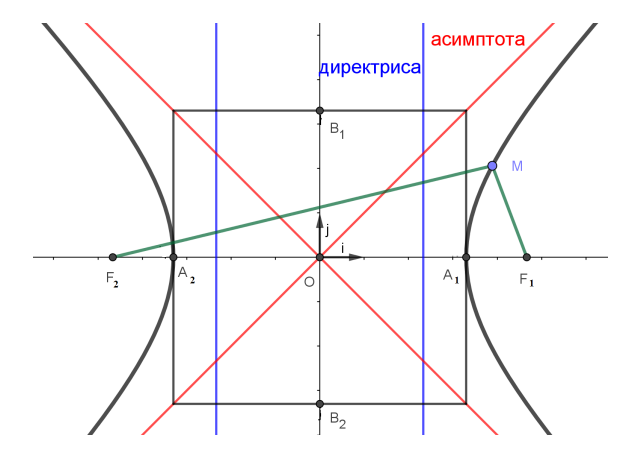
\includegraphics[height = 7cm]{images/second_hyperbola.png}
  \caption{Гипербола. $OA_1 = OA_2 = a$}
  \label{fig:hyperbola}
\end{figure}

Введём число $c$, положив
$$
  c^2 = a^2 + b^2
$$ и $c > 0$. \textit{Фокусами} гиперболы называются точки $F_1$ и $F_2$ с координатами $(c, 0)$ и $(-c, 0)$. Расстояние между ними называется \textit{фокальным расстоянием}.

Если точка $M$ "--- точка данной гиперболы, то отрезки $F_1M$ и $F_2M$ называются \textit{фокальными радиусами} точки $M$. Их длины также называются фокальными радиусами точки $M$.

\begin{theorem}
  Для того чтобы точка $M$ лежала на гиперболе необходимо и достаточно, чтобы разность её расстояний до фокусов по абсолютной величине равнялась $2a$.
\end{theorem}
\begin{Proof}
  $\Rightarrow$ Пусть $M$ удовлетворяет уравнению \ref{eq:hyperbola}. Тогда
    $$
    F_1M = \sqrt{(x - c)^2 + y^2}, ~ F_2M = \sqrt{(x + c)^2 + y^2}.
    $$
    Подставив значение $y^2$ из уравнения \ref{eq:hyperbola} и учитывая, что $c^2 = a^2 + b^2$, получим:
    \begin{gather*}
      F_1M = \sqrt{(\frac{c}{a}x - a)^2} = \mathopen|\frac{c}{a}x - a \mathclose| \\
      F_2M = \sqrt{(\frac{c}{a}x + a)^2} = \mathopen|\frac{c}{a}x + a \mathclose|
    \end{gather*}
    Так как $\mathopen|x\mathclose| \geq a, ~ \frac{c}{a} > 1$, то 
    $$
    \begin{array}{ccc}
      F_1M = \frac{c}{a}x - a, & F_2M = \frac{c}{a}x + a, & \text{при }x > 0 \\
      F_1M = -\frac{c}{a}x + a, & F_2M = -\frac{c}{a}x - a, & \text{при }x < 0 
    \end{array}
    $$
    То есть $\mathopen|F_1M - F_2M\mathclose| = 2a$.

  $\Leftarrow$ Пусть $\mathopen|F_1M - F_2M\mathclose| = 2a$. Тогда
  $$
    \mathopen| \sqrt{(\frac{c}{a}x - a)^2} - \sqrt{(x + c)^2 + y^2} \mathclose| = 2a
  $$
  Запишем это уравнение в виде 
  $$
  \mathopen| \sqrt{(\frac{c}{a}x - a)^2} = \sqrt{(x + c)^2 + y^2} \mathclose| \pm 2a
  $$
  Возводя его в квадрат и приводя подобные члены, получим:
  $$
    \pm a \sqrt{(x - c)^2 + y^2} = a^2 - xc
  $$
  Снова возводя в квадрат, после преобразований получим:
  $$
    \frac{x^2}{a^2} - \frac{y^2}{b^2} = 1
  $$
\end{Proof}
Теперь можно дать определение гиперболы:
\begin{definition}
  \textit{Гиперболой} называется множество всех точек плоскости, абсолютное значение разности расстояний каждой из которых от двух данных точек $F_1$ и $F_2$ равно длине данного отрезка $PQ$, причем $PQ < F_1F_2$.
\end{definition}


Гипербола имеет один центр симметрии и две оси симметрии. Центр симметрии совпадает с серединой фокального отрезка. Прямая, проходящая через фокусы, называется первой или фокальной осью симметрии, а перпендикулярная к ней ось "--- второй или мнимой осью симметрии. Фокальная ось
симметрии пересекает гиперболу в двух точках $A_1$ и $A_2$. Вторая ось симметрии не пересекает гиперболу. Точки $A_1$ и $A_2$ называются вершинами гиперболы, отрезок
$A_1A_2 = 2a$ — \textit{действительной} осью. Отрезок $2b$ — \textit{мнимой} осью. Числа $a$ и $b$
называются соответственно \textit{действительной} и \textit{мнимой полуосями} гипербол.

Гипербола \ref{eq:hyperbola} состоит из двух \textit{ветвей} (правой и левой) и расположена
симметрично относительно осей координат.

Отношение
$$
  e = \frac{c}{a}
$$ называется \textit{эксцентриситетом} гиперболы.

Так как $a < c$, то $e > 1$.

Выясним, как зависит форма гиперболы от её эксцентриситета. Так как $c^2 = a^2 + b^2$ получаем: $\frac{b}{a} =\sqrt{e^2 - 1}$ или $\operatorname{tg}\, \alpha = \sqrt{e^2 - 1}$
где $\alpha$ – угол между осью
абсцисс и асимптотой. Отсюда следует, что больше эксцентриситет, тем больше $\alpha$, т.е. тем больше гипербола <<вытянута>> вдоль своей мнимой оси.

Расстояние от произвольной точки $M(x,y)$ вычисляется:
\begin{itemize}
  \item Если $M$ принадлежит правой ветке: $r_1 = ex - a$, $r_2 = ex + a$.
  \item Если $M$ принадлежит левой ветке: $r_1 = -ex + a$, $r_2 = -ex - a$.
\end{itemize}
В общем виде это можно записать так:
$$
  r_1 = \mathopen|ex - a\mathclose| \text{ и } r_2 = \mathopen|ex + a\mathclose|
$$

\begin{definition}
  \textit{Директрисами гиперболы} называются две прямые, перпендикулярные фокальной оси и отстоящие от центра на расстоянии, равном $\frac{a}{e}$.

  Уравнения директрис $d_1$ и $d_2$ следующие: $x = \pm \frac{a}{e}$.
\end{definition}
Для того, чтобы точка лежала на
гиперболе, необходимо и достаточно, чтобы отношение ее
расстояния до фокуса к расстоянию до соответствующей
директрисы равнялось эксцентриситету $e$.

Гипербола также имеет две асимптоты, уравнения которых $y = \pm \frac{b}{a}x$. На асимптотах лежат диагонали прямоугольника, центр которого совпадает с центром
гиперболы, а стороны равны и параллельны осям гиперболы.

Произведение расстояний от точки гиперболы до асимптот постоянно и равно $\frac{a^2b^2}{a^2 + b^2}$

Гипербола, полуоси которой равны $(a = b)$, называется \textit{равносторонней}. Ее каноническое уравнение имеет вид: $x^2 - y^2 = a^2$.

\begin{definition}
  Гипербола, задаваемая уравнением
  $$
    -\frac{x^2}{a^2} + \frac{y^2}{b^2} = 1
  $$
  называется \textit{сопряженной} с гиперболой, задаваемой с уравнением \ref{eq:hyperbola}. Она пересекает ось $Oy$ в точках $B_1(b,0), \; B_2(-b, 0)$, не пересекает ось $Ox$, так что $a$ "--- ее мнимая полуось, а $b$ "--- действительная.
\end{definition}

Касательная к гиперболе, задаваемая уравнением \ref{eq:hyperbola}, в точке $(x_0; y_0)$ определяется уравнением:
$$
  \frac{xx_0}{a^2} - \frac{yy_0}{b^2} = 1
$$

\subsection*{Парабола}
Параболой по теореме \ref{theorem:second} была названа линия, которая в некоторой прямоугольной системе координат определяется каноническим уравнением:
\begin{equation}
  \label{eq:parabola}
  y^2 = 2px
\end{equation} при условии $p > 0$.

Из уравнения \ref{eq:parabola} вытекает, что для всех точек параболы выполняется $$\begin{cases}
  x \geq 0,& \text{если } p > 0 \\
  x \leq 0,& \text{если } p < 0
\end{cases}$$.
\begin{figure}[H]
  \centering
  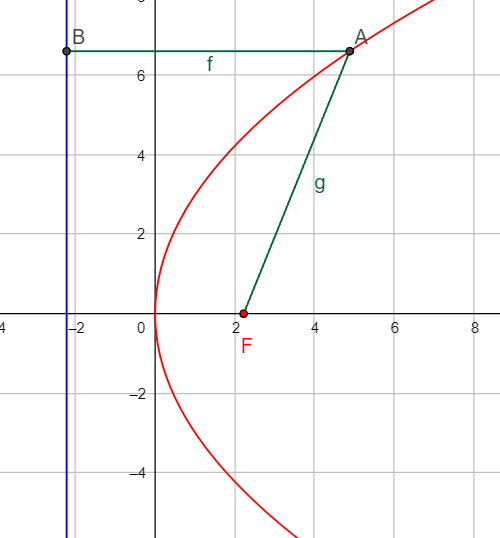
\includegraphics[height = 7cm]{images/second_parabola.png}
  \label{fig:parabola}
\end{figure}

\textit{Фокусом} параболы называется точка $F$ с координатами $(p / 2, 0)$

\textit{Директрисой} параболы называется прямая $d$ с уравнением $x = -\frac{p}{2}$

\begin{theorem}
  Для того, чтобы точка $M$ лежала
  на параболе, необходимо и достаточно, чтобы она была одинаково удалена от фокуса и от директрисы этой параболы.
\end{theorem}
\begin{Proof}
  $\Rightarrow$ Пусть $M$ удовлетворяет уравнению \ref{eq:parabola}. Тогда
  \begin{gather*}
    \rho (M, d) = \mathopen|x + \frac{p}{2}\mathclose| \\
    MF = \sqrt{(x - \frac{p}{2})^2 + y^2} = \\
    = \sqrt{(x - \frac{p}{2})^2 + 2px} = \sqrt{(x + \frac{p}{2})^2} =  \\
    = \mathopen|x + \frac{p}{2}\mathclose| = \rho (M, d)
  \end{gather*}
  $\Leftarrow$ Пусть $M$ одинаково удалена от фокуса и от директрисы параболы:
  $$
    \sqrt{(x - \frac{p}{2})^2 + y^2} = \mathopen|x + \frac{p}{2}\mathclose|
  $$
  Возводя обе части в квадрат, получаем $y^2 = 2px$.
\end{Proof}
Дадим определение параболе.
\begin{definition}
  Параболой называется множество всех точек плоскости, расстояние каждой из которых до данной точки равно расстоянию до данной прямой $d$, не проходящей через точку $F$.
\end{definition}
Парабола имеет одну ось симметрии, которая совпадает, при таком выборе системы координат, с осью $x$. При $p > 0$ парабола обращается в положительную сторону оси, а при $p < 0$ — в отрицательную. Точка $(0,0)$ называется \textit{вершиной} параболы.

Расстояние от
точки $M(x, y)$, лежащей на параболе, до
фокуса равно
$$
  r = x + \frac{p}{2}
$$

Параболе приписывается эксцентриситет e = 1. В силу этого соглашения формула
$$
  \frac{r}{d} = e,
$$ где $r$ "--- расстояние до фокуса, а $d$ расстояние до директрисы, верна и для параболы, и для гиперболы, и для эллипса.

Касательная к параболе $y^2 = 2px$ в точке $(x_0; y_0)$ определяется уравнением:
$$
  yy_0 = p(x + x_0).
$$

\subsection*{Директориальное свойство}
\begin{definition}
  Директрисами эллипса (гиперболы) называются две прямые, параллельные малой (мнимой) оси и отстоящие от неё на расстоянии $\frac{a}{e}$, где $a$ -
  большая (действительная) полуось, $e$ - эксцентриситет.
\end{definition}

Окружность не имеет директрис, так как для неё $e = 0$.

Директрисы \textit{эллипса} \textbf{не имеют} общих точек с большой осью эллипса,
они не пересекают эллипс.

Директрисы \textit{гиперболы} \textbf{пересекают} вещественную ось гиперболы, они
расположены между двумя ветвями гиперболы и не пересекают эти ветви.

\begin{theorem}
  Эллипс (гипербола) есть множество $\gamma'$
  всех точек плоскости таких, что отношение расстояния от каждой точки до фокуса к
  расстоянию от неё до соответствующей директрисы равно эксцентриситету.
\end{theorem}

\begin{Proof}
  Пусть $\gamma$ "--- данный эллипс, 
  
  $F_1(c, 0)$ "--- фокус, 
  
  $d_1: ~  x = \frac{a}{e}$ "--- директриса.

  Если $M(x, \, y)$ "--- точка плоскости, то
  $$
     \rho  (M, \, d_1) = \mathopen|x - \frac{a}{e}\mathclose|, ~ MF_1  = \sqrt{(x - c)^2 + y^2}
  $$

  Если $M \in \gamma'$, то $\sqrt{(x - c)^2 + y^2} = e \mathopen|x - \frac{a}{e}\mathclose|$. Возводя то уравнение в квадрат, получим:
  \begin{gather*} 
    (x - c)^2 + y^2 = (ex - a)^2 \implies x^2 - 2xc + c^2 + y^2 = (ex)^2 - 2exa + a^2 \implies \\
    x^2(1 - e^2) + y^2 = 2xc - c^2 - 2xa \frac{c}{a} + a^2 \implies x^2 (1 - \frac{c^2}{a^2}) + y^2 = a^2 - c^2 \implies \\
    x^2 \frac{b^2}{a^2} + y^2 = b^2 \implies \frac{x^2}{a^2} + \frac{y^2}{b^2} = 1
  \end{gather*}
  Отсюда следует, что $M \in \gamma$.

  Обратно, пусть $M(x, \, y) \in \gamma$, значит, координаты точки удовлетворяют уравнению эллипса $\frac{x^2}{a^2} + \frac{y^2}{b^2} = 1$. Тогда
  \begin{gather*}
    MF_1 = \sqrt{(x - c)^2 + y^2} = \sqrt{(x - c)^2 + b^2 (1 - \frac{x^2}{a^2})} = \\
    = \sqrt{(x - c)^2 + (a^2 - c^2)(1 - \frac{x^2}{a^2})} = \sqrt{x^2 - 2xc + c^2 + a^2 - c^2 - (a^2 - c^2)\frac{x^2}{a^2}} = \\
    = \sqrt{x^2 - 2xc + a^2 - x^2 + c^2 \frac{x^2}{a^2}} = \sqrt{(a - \frac{c}{a}x)^2} = \\
    = \sqrt{(a - ex)^2} = \mathopen|a - ex\mathclose|.
  \end{gather*}
  Так как $\mathopen|x\mathclose| \leq a$ и $0 < \frac{c}{a} < 1$, то $a - \frac{c}{a}x = a - ex > 0$, поэтому
  $$
    MF_1 = a - ex.
  $$

  С другой стороны, $\rho (M, \, d_1) = \mathopen|x - \frac{a}{e}\mathclose| = \frac{a - ex}{e},$ поэтому $MF_1 = e\rho(M, \, d_1)$, то есть $M \in \gamma'$. Множество $\gamma'$ совпадает с эллипсом $\gamma$.
  
  Теорема для гиперболы доказывается точно так же, как и для эллипса.
\end{Proof}

Эта теорема выясняет геометрический смысл эксцентриситета эллипса
или гиперболы: эксцентриситет эллипса или гиперболы есть то постоянное
число, которому равно отношение расстояний от каждой точки линии до фокуса к расстоянию от нее до соответствующей директрисы. Из определения
параболы видно, что её точки обладают аналогичным свойством, т.е. отношение от каждой точки параболы до фокуса к расстоянию от неё до директрисы
постоянно и равно единице.

\subsection*{Поверхности второго порядка}
\begin{definition}
  
  В аффиной системе координат общее уравнение поверхности второго порядка имеет вид:
  \begin{align}
    \label{eq:second_plane}
    F(x,y,z) = a_{11}x^2 + a_{22}y^2 + a_{33}z^2 + 2a_{12}xy + 2a_{13}&xz + 2a_{23}yz+\\ + 2a_{10}x + 2a_{20}y +2a_{30}z + a_{00} = 0. \nonumber
  \end{align}
\end{definition}

Коэффициенты этого уравнения "--- любые действительные числа, причем $a_{11}, \, a_{22}, \, a_{33}, \, a_{12}, \, a_{13}, \, a_{23}$ не равны одновременно нулю.

$\begin{pmatrix}
  a_{11} & a_{22} & a_{13} \\
  a_{21} & a_{22} & a_{23} \\
  a_{31} & a_{32} & a_{33} 
\end{pmatrix}$ "--- матрица \textit{квадратной} части ($a_{12} = a_{21}, \; a_{13} = a_{31}, \; a_{23} = a{32}$),
$\begin{pmatrix} a_{10} & a_{20} & a{30} \end{pmatrix}$ "--- матрица \textit{линейной} части.

Уравнение \ref{eq:second_plane} можно записать в виде:
$$
  F(x,y,z) = \begin{pmatrix} x & y & z \end{pmatrix} \cdot \begin{pmatrix}
    a_{11} & a_{22} & a_{13} \\
    a_{21} & a_{22} & a_{23} \\
    a_{31} & a_{32} & a_{33}
  \end{pmatrix} \cdot \begin{pmatrix}
    x \\ y \\ z
  \end{pmatrix} + 2 \begin{pmatrix}
    a_{10} & a_{20} & a_{30}
  \end{pmatrix} \cdot \begin{pmatrix}
    x \\ y \\ z
  \end{pmatrix} + a_{00} = 0.
$$

\begin{theorem}
  Для любой поверхности второго порядка существует прямоугольная система координат, в которой она имеет один из следующих 17 видов:
  \begin{enumerate}
    \item Эллипсоид $$
      \frac{x^2}{a^2} + \frac{y^2}{b^2} + \frac{z^2}{c^2} = 1, ~(a \geq b \geq c > 0)
    $$
    \item Мнимый эллипсоид $$
      \frac{x^2}{a^2} + \frac{y^2}{b^2} + \frac{z^2}{c^2} = -1, ~(a \geq b \geq c > 0)
    $$
    \item Однополостный гиперболоид $$
      \frac{x^2}{a^2} + \frac{y^2}{b^2} - \frac{z^2}{c^2} = 1, ~(a \geq b > 0)
    $$
    \item Двуполостный гиперболоид $$
      -\frac{x^2}{a^2} - \frac{y^2}{b^2} + \frac{z^2}{c^2} = 1, ~(a \geq b > 0)
    $$
    \item Конус (второго порядка) $$
      \frac{x^2}{a^2} + \frac{y^2}{b^2} - \frac{z^2}{c^2} = 0, ~(a \geq b > 0)
    $$
    \item Мнимый конус (второго порядка) $$
      \frac{x^2}{a^2} + \frac{y^2}{b^2} + \frac{z^2}{c^2} = 0, ~(a \geq b > 0)
    $$
    \item Эллиптический параболоид $$
      \frac{x^2}{p} + \frac{y^2}{q} = 2z, ~(p \geq q > 0)
    $$
    \item Гиперболический параболоид $$
      \frac{x^2}{p} - \frac{y^2}{q} = 2z, ~(p \geq q > 0)
    $$
    \item Эллиптический цилиндр $$
      \frac{x^2}{a^2} + \frac{y^2}{b^2} = 1, ~(a \geq b > 0)      
    $$
    \item Мнимый эллиптический цилиндр $$
      \frac{x^2}{a^2} + \frac{y^2}{b^2} = -1, ~(a \geq b > 0)      
    $$
    \item Гиперболический цилиндр $$
    \frac{x^2}{a^2} - \frac{y^2}{b^2} = 1, ~(a \geq b > 0)      
    $$
    \item Параболический цилиндр $$
    y^2 = 2px, ~ (p > 0)
    $$
    \item Две пересекающиеся плоскости $$
    \frac{x^2}{a^2} - \frac{y^2}{b^2} = 0, ~(a \geq b > 0)      
    $$
    \item Две мнимые пересекающие плоскости $$
      \frac{x^2}{a^2} + \frac{y^2}{b^2} = 0, ~(a \geq b > 0)      
    $$
    \item Две параллельные плоскости $$
    y^2 = a^2, ~ (a > 0)
    $$
    \item Две мнимые параллельные плоскости $$
      y^2 = -a^2, ~ (a > 0)
    $$
    \item Две совпадающие плоскости $$
      y^2 = 0
    $$
  \end{enumerate}
\end{theorem}

\subsection*{Метод сечений}

\textit{Метод сечений} применим к любой поверхности, а не только к поверхности второго порядка. Сущность метода сечений состоит в следующем.

Пусть поверхность $S$ задана в прямоугольной системе координат уравнением $F(x, y, z) = 0$. Поверхность $S$ пересекаем плоскостями, параллельными
коориднатным плоскостям (или самими координатными плоскостями), и находим линии пересечения поверхности с этими плоскостями. По виду этих
линий сечений выносится суждение о форме поверхности $S$.

\begin{example}
  Определите поверхность, которая задана в прямоугольной системе координат уравнением $$
    \frac{x^2}{16} - \frac{y^2}{9} + \frac{z^2}{4} = 1.
  $$

  Найдем пересечение поверхности с плоскостью $xOy$.
  $$
  \begin{array}{cccc}
    \begin{cases}
      \frac{x^2}{16} - \frac{y^2}{9} + \frac{z^2}{4} = 1 \\
      z = 0
    \end{cases} &
    \Leftrightarrow &
    \begin{cases}
      \frac{x^2}{16} - \frac{y^2}{9}  = 1 \\
      z = 0
    \end{cases} &
    \text{Гипербола} 
  \end{array}
    $$
    
    Найдем пересечение поверхности с плоскостью $xOz$.
    $$
    \begin{array}{cccc}
      \begin{cases}
        \frac{x^2}{16} - \frac{y^2}{9} + \frac{z^2}{4} = 1 \\
        y = 0
      \end{cases} &
      \Leftrightarrow &
      \begin{cases}
        \frac{x^2}{16} - \frac{y^2}{9}  = 1 \\
        y = 0
      \end{cases} &
      \text{Эллипс} 
    \end{array}
      $$

    Найдем пересечение поверхности с плоскостью $yOz$.
    $$
    \begin{array}{cccc}
      \begin{cases}
        \frac{x^2}{16} - \frac{y^2}{9} + \frac{z^2}{4} = 1 \\
        x = 0
      \end{cases} &
      \Leftrightarrow &
      \begin{cases}
         - \frac{y^2}{9}  = 1 \\
        x = 0
      \end{cases} &
      \text{Гипербола} 
    \end{array}
      $$

    Изобразив каждую фигуру второго порядка в соответсвтующих плоскостях, получим, что исходное уравнение "--- однополостный гиперболоид.
\end{example}

\subsection*{Поверхности вращения}
\begin{definition}
  Поверхность, которая вместе с каждой своей точкой содержит всю окружность, полученную вращением этой точки вокруг некоторой фиксированной прямой $d$, называется \textit{поверхностью вращения}.

  Прямая $d$, вокруг которой производится вращение, называется \textit{осью вращения}.
\end{definition}

Вращение точки вокруг оси происходит в плоскости, перпендикулярной оси.

В сечении поверхности вращения плоскостями, перпендикулярными оси вращения, получаются окружности, которые называются \textit{параллелями}.

Плоскости, проходящие через ось вращения, пересекают поверхность вращения по линиям, называемыми \textit{меридианами}.

\begin{definition}
  В прямоугольной системе координат $O\bar{i}\bar{j}\bar{k}$ уравнение $$
    x^2 + y^2 = f^2(z)
  $$
  есть уравнение поверхности вращения, образованной вращением вокруг оси $Oz$ линии, заданной уравнениями: $$
    x = f(z), ~ y = 0.
  $$
\end{definition}

Аналогично можно рассмотреть все остальные случаи расположения линии в координатных плоскостях и её вращения вокруг соответствующих осей.

\begin{table}[H]
  \centering
  \begin{tabular}{|p{1cm}|p{2cm}|p{2cm}|p{2cm}|p{4cm}|}
  \hline
      № & Линия $\gamma$ лежит в плоскости & Линия $\gamma$ задается уравнением
      & Линия $\gamma$
      вращается
      вокруг оси
       & Уравнение поверхности вращения \\ \hline
      1 & $Oxz$& $x = f(z)$ & $Oz$ & $x^2 + y^2 = (f(z))^2$ \\ \hline
      2 & $Oxz$ & $z = f_1(x)$ & $Ox$ & $y^2 + z^2 = (f_1(z))^2$ \\ \hline
      3 & $Oxy$ & $x = g(y)$ & $Oy$ & $x^2 + z^2 = (g(y))^2$ \\ \hline
      4 & $Oxy$ & $y = g_1(y)$ & $Ox$ & $y^2 + z^2 = (g_1(x))^2$ \\ \hline
      5 & $Oyz$ & $y = h(z)$ & $Oz$ & $x^2 + y^2 = (h(z))^2$ \\ \hline
      6 & $Oyz$ & $z = h_1(y)$ & $Oy$ & $x^2 + z^2 = (h_1(y))^2$ \\ \hline
  \end{tabular}
\end{table}

\begin{example}
  В плоскости $Oxz$ прямоугольной системе координат $Oxyz$ дана окружность $x^2 + z^2 = r^2$ с центром в начале координат радиуса $r$. Написать уравнение поверхности $S$, образованной вращением этой окружности вокруг оси $Oz$.

  Сначала получим уравнение линии $\gamma$, в результате вращения которой вокруг оси $Oz$ образуется поверхность. Из уравнения данной окружности находим: $x = \pm \sqrt{r^2 - z^2}$.

  Здесь знаку <<$+$>> соответствует одна полуокружность, а знаку <<$-$>> "--- другая полуокружность данной окружности. Ясно, что при вращении вокруг
  оси $Oz$ каждой из этих полуокружностей получается та же поверхность, что и вращении всей окружности.

  Поэтому в качестве линии $\gamma$ можно взять одну из указанных полуокружностей, например,
  $$
    x = \sqrt{r^2 - z^2},~ y = 0
  $$

  Уравнение поверхности $S$ имеет вид: $$
    x^2 + y^2 = (\sqrt{r^2 - z^2})^2 \leftrightarrow x^2 + y^2 + z^2 = r^2.
  $$

  Таким образом, поверхностью $S$ является сфера $r$ с центром в начале координат.
\end{example}

\begin{example}
  В плоскости $Oxz$ прямоугольной системе координат $Oxyz$ дана прямая $x = a$, параллельная оси $Oz$. Написать уравнение поверхности,
  образованной вращением этой прямой вокруг оси $Oz$.
  
  Уравнение направляющей: $x = a, \; y = 0$.

  Тогда поверхность вращения определяется уравнением $x^2 + y^2 = a^2$.
  Эта поверхность называется цилиндром вращения (или прямым круговым цилиндром).
  \begin{figure}[H]
    \centering
    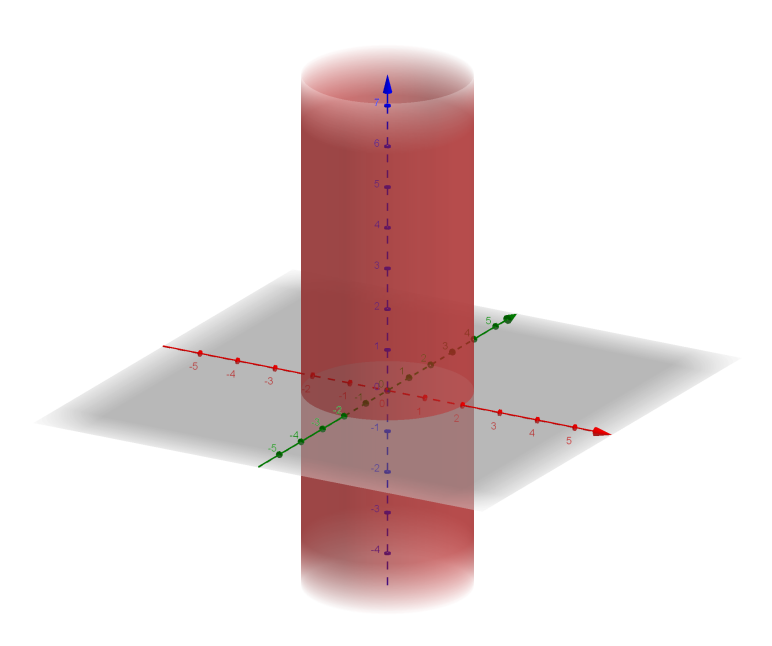
\includegraphics[height = 4cm]{images/second_сylinder.png}
  \end{figure}
\end{example}

\begin{example}
  Пусть линия $\gamma$ представляет собой эллипс, лежащий в координатной плоскости $Oxz$ и задаваемый каноническим уравнением $\frac{x^2}{a^2} + \frac{z^2}{c^2} = 1$.

  Чтобы составить уравнение поверхности, получаемой вращением этого эллипса вокруг оси $Ox$, надо разрешить уравнение относительно $z$: $$
    z = \pm c \sqrt{1 - \frac{x^2}{a^2}}
  $$
  
  Тогда уравнение поверхности вращения имеет вид:$$
    y^2 + z^2 = (\pm \sqrt{1 - \frac{x^2}{a^2}})^2 \Leftrightarrow y^2 + z^2 = c^2(1 - \frac{x^2}{a^2}) \Leftrightarrow \frac{x^2}{a^2} + \frac{y^2}{c^2} + \frac{z^2}{c^2} = 1.
  $$

  Если данный эллипс вращается вокруг оси $Oz$, то уравнение эллипса нужно разрешить относительно
  $x$ и прийти к следующему уравнению поверхности вращения: $$
    \frac{x^2}{a^2} + \frac{y^2}{a^2} + \frac{z^2}{c^2} = 1
  $$
  
  Каждая из этих поверхностей называется эллипсоидом вращения.
  \begin{figure}[H]
    \centering
    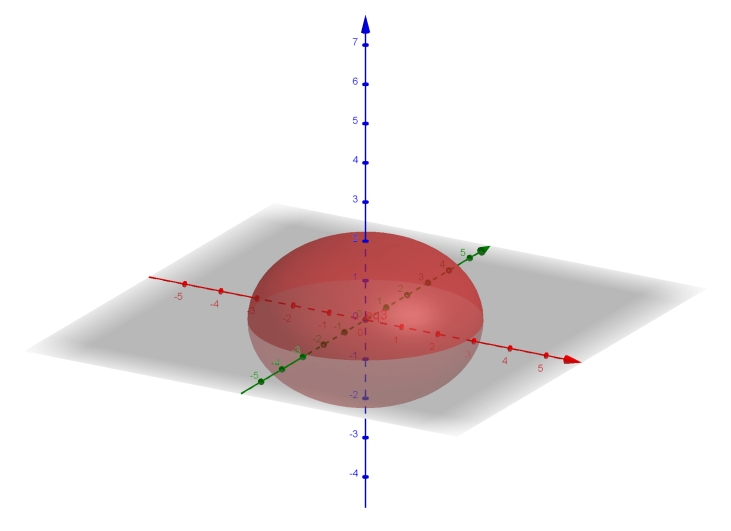
\includegraphics[height = 4cm]{images/second_ellipsoid.png}
  \end{figure}
\end{example}

\subsection*{Конические поверхности}

Рассмотрим поверхность, определяемую в некоторой декартовой системе координат уравнением $F(x, y, z)=0$. Если точка $M$ с координатами
$(x, y, z)$ принадлежит поверхности, то при любом $\lambda$ точка $P(\lambda x, \lambda y, \lambda z)$ также принадлежит поверхности.
\begin{definition}
  Поверхность, которая состоит из прямых линий, проходящих через фиксированную точку, называется \textit{конической поверхностью} или \textit{конусом}. 
  
  Прямые линии называются ее \textit{образующими}, а точка — \textit{вершиной конуса}. 
  
  Линию, лежащую на поверхности, не проходящую
  через вершину и пересекающую все образующие, называют
  \textit{направляющей}.
\end{definition}

\begin{figure}[H]
  \centering
  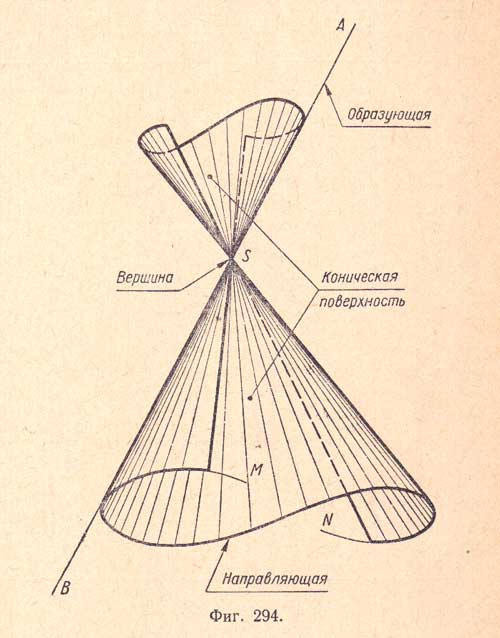
\includegraphics[height = 7cm]{images/second_conical.jpg}
\end{figure}

Напомним уравнение конуса второго порядка: 
$$
  \frac{x^2}{a^2} + \frac{y^2}{b^2} - \frac{z^2}{c^2} = 0, ~ (a \geq b > 0)
$$

\subsection*{Цилиндрические поверхности}

Пусть точка $M_0(x_0, y_0, z_0)$
лежит на поверхности. Тогда все точки с координатами
$x_0, y_0, z$ при любых $z$ также
лежат на поверхности. 
\begin{definition}
  Поверхность, которая состоит из прямых линий, параллельных заданному направлению, называется \textit{цилиндрической поверхностью} или \textit{цилиндром}, а прямые линии — ее \textit{образующими}.
  
  Линию, лежащую на поверхности и пересекающую все образующие, называют \textit{направляющей}.
\end{definition}

\begin{figure}[H]
  \centering
  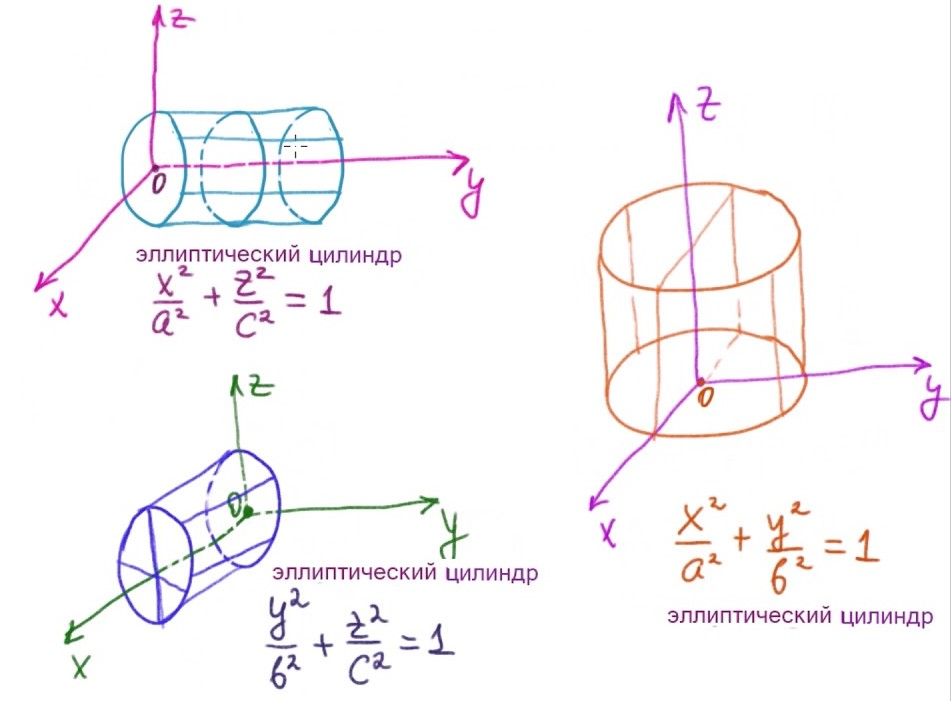
\includegraphics[height = 6cm]{images/second_cylinder_surface.jpg}
\end{figure}

\subsection*{Эллипсоид}
Поверхность с уравнением $$
  \frac{x^2}{a^2} + \frac{y^2}{b^2} + \frac{z^2}{c^2} = 1
$$ называется эллипсоидом.

Эллипсоид получается вращением эллипса вдоль малой оси эллипса либо большой оси.
\begin{figure}[H]
  \centering
  \begin{subfigure}[b]{0.4\textwidth}
    \centering
    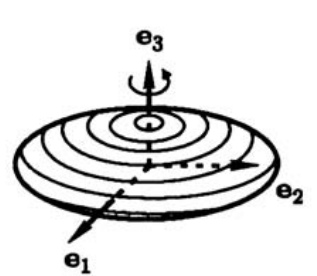
\includegraphics[width = \textwidth]{images/second_ellipsoid_A.png}
  \end{subfigure}
  \hfill
  \begin{subfigure}[b]{0.4\textwidth}
    \centering
    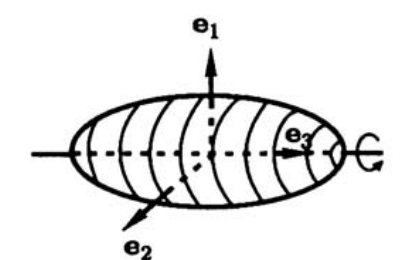
\includegraphics[width = \textwidth]{images/second_ellipsoid_B.png}
  \end{subfigure}
\end{figure}

\subsection*{Однополостный гиперболоид}

Однополостный гиперболоид вращения "--- это поверхность вращения гиперболы вокруг той оси, которая ее не пересекает.
\begin{figure}[H]
  \centering
  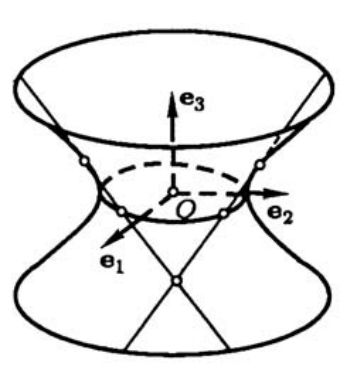
\includegraphics[height = 4cm]{images/second_hyperboloid_one.png}
\end{figure}
Интересное свойство однополостного гиперболоида — наличие у него \textit{прямолинейных образующих}. Так называются прямые линии, всеми своими точками лежащие на поверхности. Через каждую точку однополостного гиперболоида проходят две прямолинейные образующие, уравнения которых можно получить следующим образом. Уравнения этих образующих следующие: $$
  x + y = 1 - z, ~~ x - y = 1 - z. 
$$

Если вместе с гиперболой мы будем вращать ее асимптоты, то они опишут прямой круговой конус, называемый \textit{асимптотическим конусом} гиперболоида вращения.

\subsection*{Двуполостный гиперболоид}
Двуполостный гиперболоид вращения — это поверхность получаемая вращением
гиперболы вокруг той оси, которая ее пересекает.
\begin{figure}[H]
  \centering
  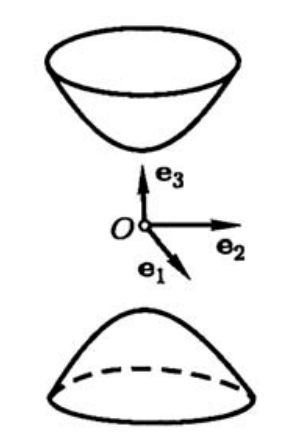
\includegraphics[height = 4cm]{images/second_hyperboloid_two.png}
\end{figure}

\subsection*{Эллиптический параболоид}
Вращая параболу $x^2 = 2pz$ вокруг ее
оси симметрии, мы получаем поверхность, которая называется эллиптическим параболоидом.
\begin{figure}[H]
  \centering
  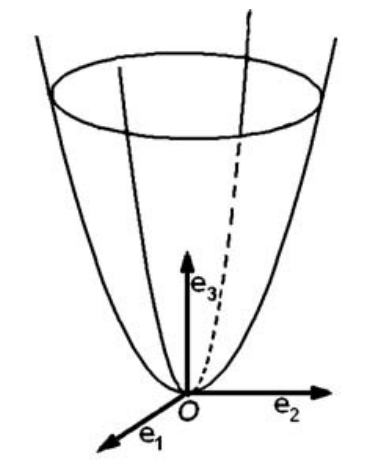
\includegraphics[height = 4cm]{images/second_ellipsoid_parabola.png}
\end{figure}

\subsection*{Гиперболический параболоид}
Поверхность с уравнением $$
  \frac{x^2}{p} - \frac{y^2}{q} = 2z, ~ (p \geq q > 0).
$$
\begin{figure}[H]
  \centering
  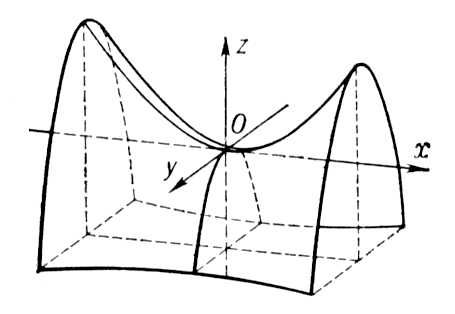
\includegraphics[height = 4cm]{images/second_hyperboloid_parabola.jpg}
\end{figure}

Построить гиперболический параболоид можно
следующим образом: зададим две параболы и будем перемещать одну из них так, чтобы ее вершина скользила по другой, оси парабол были параллельны, параболы лежали во взаимно перпендикулярных плоскостях и ветви их были направлены в противоположные стороны. При таком перемещении
подвижная парабола описывает гиперболический параболоид

Гиперболический параболоид, как и однополостный гиперболоид, имеет два семейства прямолинейных образующих. Уравнения одного семейства $$
  \lambda (\frac{x}{a} - \frac{y}{b}) = \mu, ~~ \mu (\frac{x}{a} + \frac{y}{b}) = 2\lambda z,
$$
а другого  $$
  \lambda'(\frac{x}{a} + \frac{y}{b}) = \mu'. ~~
  \mu'(\frac{x}{a} - \frac{y}{b}) = 2\lambda'z,
$$ "--- где $\lambda$ и $\mu$ произвольные параметры.

\subsection*{Приведение общего уравнения второго порядка на плоскости и в пространстве к каноническому виду}
(если будет выполнено домашнее задание, этот вопрос не нужно учить)

404

\end{document}